\documentclass[11pt]{article}

\usepackage[margin=1.1in]{geometry}
\usepackage{amsmath,amssymb}
\usepackage{graphicx}
\usepackage{booktabs}
\usepackage[round]{natbib}
\usepackage{xcolor}
\usepackage[colorlinks=true,linkcolor=blue!60!black,citecolor=blue!60!black,urlcolor=blue!60!black]{hyperref}
\usepackage{fancyhdr}

\graphicspath{{../figures/}}

\pagestyle{fancy}
\fancyhf{}
\fancyhead[L]{\textcolor{red!70!black}{\textsc{working draft --- not for distribution}}}
\fancyhead[R]{\thepage}

\newcommand{\dsob}{\Delta_{\mathrm{Sob}}}
\newcommand{\taus}{\tau_{\mathrm{S}}}
\newcommand{\kms}{\,\mathrm{km\,s^{-1}}}
\newcommand{\todo}[1]{\textcolor{red}{[TODO: #1]}}

\title{How Large Is the Error of the Sobolev-Class Line-Transfer
Approximation in Kilonova Ejecta?\\[4pt]
\large I. A controlled three-way validation harness and first validity-map
measurements with calibrated La\,\textsc{ii} atomic data}
\author{Yonglin Zhu}
\date{August 15, 2026 --- working draft}

\begin{document}
\maketitle

\begin{abstract}
\noindent
The light emitted by a kilonova---the radioactive glow of matter ejected when
two neutron stars merge---must pass through a gas containing millions of
absorption lines of freshly synthesized heavy elements. Simulating this is so
expensive that essentially all kilonova radiative-transfer codes replace the
true, frequency-resolved interaction of light with each line by a shortcut
built on the \emph{Sobolev approximation}, most commonly in its binned
``expansion opacity'' form. This paper series asks a simple question that is
rarely answered quantitatively: \emph{how large is the error of that
shortcut, and where in kilonova parameter space does it matter?}
We construct a deliberately small, fully controlled test harness in which the
same ejecta model, the same atomic data, and the same level populations are
pushed through three independent calculations: an analytic Sobolev
prediction, a deterministic frequency-resolved reference solver written for
this work, and the Monte Carlo code \textsc{sedona}, which implements both a
resolved line treatment and the expansion-opacity treatment. The three
resolved-physics calculations agree to $\sim1\%$ once a thermal-emission
convention is matched, in every experiment from a single artificial line to a
realistic forest of 153 calibrated La\,\textsc{ii} lines from the GSI
kilonova atomic database. Against this validated baseline we separate two
errors that the literature conflates under a single name. The
\emph{expansion-opacity implementation} carries a strength-set error floor,
arising from a per-resonance substitution $\tau \to 1-e^{-\tau}$, that grows
from $\sim3\%$ for weak-line forests to $40$--$90\%$ for strong-line forests
and survives undiminished down to a Doppler width of $1\kms$---essentially
the thermal width of lanthanum---so that no refinement of line widths
rehabilitates it. The \emph{Sobolev approximation itself}, by contrast, shows
no strength floor whatever and is accurate to $\approx5$--$8\%$ at
kilonova-relevant line widths; its own failure mode is the neglect of finite
line width, invisible at narrow widths and reaching $+39\%$ only for strong
lines at $300\kms$. In the strong-line, incompletely-blanketed regime where
kilonova spectral features form, the shortcut in common use is thus wrong by
tens of percent for reasons largely unrelated to the approximation it is
named after. We also report a measured cost curve for resolved transport
and several methodological findings, including an exact symmetry that makes
gradient-based Sobolev validity diagnostics systematically conservative.
\end{abstract}

\tableofcontents

%=====================================================================
\section{Introduction}
\label{sec:intro}

\subsection{Kilonovae in three paragraphs}

When two neutron stars spiral into each other and merge, a small fraction of
their matter---between roughly a thousandth and a few hundredths of a solar
mass---is flung outward at speeds of ten to thirty percent of the speed of
light. This ejected matter is one of the very few environments in the
universe dense enough in free neutrons to build the heaviest elements
(gold, platinum, uranium, and the lanthanide row of the periodic table)
through the rapid neutron-capture process, or \emph{r-process}. The
radioactive decay of these freshly made nuclei heats the expanding cloud,
which then glows for days to weeks: this glow is a \emph{kilonova}. One has
been observed in detail, AT\,2017gfo, the optical counterpart of the
gravitational-wave event GW170817 \citep{gw170817}.

Everything we want to learn from a kilonova---how much matter was ejected,
how fast, and above all \emph{which elements were made}---must be read out of
its light. The light escapes only after filtering through the ejecta, and the
filtering is dominated by an enormous number of atomic absorption lines.
Lanthanide ions are the worst offenders: because of their complex open
$4f$ electron shells, a single lanthanide ion can have tens of thousands of
energy levels and millions of radiative transitions \citep{gsi_atomic}. The
opacity of the ejecta, and therefore the color, brightness, and spectral
features of the kilonova, is controlled by these line forests.

Simulating light transport through millions of lines, each intrinsically
narrower than one part per million in frequency, is prohibitively expensive
if done directly. Every practical kilonova radiative-transfer code therefore
leans on an approximation introduced by \citet{sobolev1960} for expanding
stellar envelopes, usually packaged in the ``expansion opacity'' form of
\citet{karp1977} and \citet{eastman1993}. Section~\ref{sec:primer} explains
both ideas from scratch. The approximation is standard, venerable, and
almost never checked against a resolved calculation \emph{under kilonova
conditions}. This work begins that check.

\subsection{What this paper does}

We do not build a kilonova pipeline. We build the smallest apparatus that can
measure the approximation error cleanly, and we operate it on progressively
more realistic inputs. Concretely, this first paper reports:

\begin{itemize}
  \item a \textbf{three-way validation harness}
  (Section~\ref{sec:methods}): the same spherically expanding model, atomic
  data, and level populations evaluated by (a) analytic Sobolev theory, (b) a
  purpose-written deterministic frequency-resolved solver, and (c) the Monte
  Carlo code \textsc{sedona} \citep{sedona} in both its resolved and its
  expansion-opacity modes;
  \item \textbf{verification experiments} (Section~\ref{sec:verification})
  in which the three resolved-physics calculations agree at the
  $1$--$4\%$ level, from one artificial line to a twenty-line ladder;
  \item \textbf{measurements on real atomic data}
  (Section~\ref{sec:results}): a forest of 153 calibrated La\,\textsc{ii}
  lines from the GSI database \citep{gsi_atomic,gsi_zenodo}, and the first
  rows of a \emph{validity map}: the expansion-opacity flux error $\dsob$ as
  a function of line strength, Doppler width, and temperature;
  \item six \textbf{methodological findings} (F1--F6, collected in
  Table~\ref{tab:findings}), including an exact symmetry cancellation that
  makes gradient-based validity diagnostics conservative (F1), the
  demonstration that ``Sobolev mode'' in transport codes---i.e.\ expansion
  opacity---attenuates a single strong line by $e^{-(1-e^{-\tau})}$ rather
  than $e^{-\tau}$ (F4), and the measurement that this error is
  \emph{per-resonance} and does not average away with line count (F5) nor
  vanish in the small-line-width limit (F6).
\end{itemize}

Readers with no radiative-transfer background should read
Section~\ref{sec:primer} first; the appendix derives every formula used in
the text at a level that assumes only basic calculus.

%=====================================================================
\section{A compact radiative-transfer primer}
\label{sec:primer}

\subsection{Light through matter: intensity, opacity, optical depth}

Consider a beam of light of frequency $\nu$ traveling through a gas. Its
strength is described by the \emph{specific intensity} $I_\nu$ (energy per
unit time, area, solid angle, and frequency). Along a path length $s$, the
gas removes energy from the beam (absorption) and adds its own (emission):
\begin{equation}
  \frac{\mathrm{d}I_\nu}{\mathrm{d}s} \;=\; -\,\alpha_\nu\, I_\nu \;+\; j_\nu .
  \label{eq:rte}
\end{equation}
Here $\alpha_\nu$ (units cm$^{-1}$) is the \emph{absorption coefficient}:
$1/\alpha_\nu$ is the average distance a photon travels before being
absorbed. The emissivity $j_\nu$ describes how much the gas glows. In this
work the gas is kept in conditions where its own glow at the relevant
frequencies is negligible or exactly modeled (Section~\ref{sec:conventions}),
so absorption is the star of the show.

The dimensionless quantity that controls absorption is the
\emph{optical depth}
\begin{equation}
  \tau_\nu \;=\; \int \alpha_\nu\, \mathrm{d}s ,
  \label{eq:tau}
\end{equation}
which counts how many absorption mean-free-paths the beam crosses. If the gas
does not glow, the solution of Eq.~(\ref{eq:rte}) is simply
\begin{equation}
  I_\nu^{\rm out} \;=\; I_\nu^{\rm in}\, e^{-\tau_\nu}:
  \label{eq:beer}
\end{equation}
a beam crossing optical depth $\tau=1$ keeps $37\%$ of its light, $\tau=2$
keeps $14\%$, $\tau=5$ keeps $0.7\%$. Every result in this paper is,
at bottom, a statement about which $\tau$ gets exponentiated.
(The full solution with emission is derived in Appendix~\ref{app:formal}.)

\subsection{Spectral lines and Doppler width}

Atoms absorb light most strongly at the discrete frequencies of their
internal transitions---\emph{spectral lines}. A line is not infinitely
sharp: thermal motion of the absorbing ions Doppler-shifts each ion's
absorption slightly, smearing the line into a profile $\phi(\Delta\nu)$
(normalized so $\int\phi\,\mathrm{d}\nu = 1$) whose width corresponds to a
velocity
\begin{equation}
  v_D \;=\; \sqrt{2 k_B T / m_{\rm ion}} ,
\end{equation}
typically $\sim 0.6\kms$ for lanthanum at kilonova temperatures. Expressed
as a fraction of the line frequency this is $v_D/c \sim 2\times10^{-6}$:
lines are extraordinarily narrow. The absorption coefficient of one line is
\begin{equation}
  \alpha_\nu \;=\; \sigma_{\rm cl}\, f\, n_l\, \phi(\nu - \nu_0),
  \qquad
  \sigma_{\rm cl} \equiv \frac{\pi e^2}{m_e c} = 0.02654\ \mathrm{cm^2\,Hz},
  \label{eq:linealpha}
\end{equation}
where $\nu_0$ is the line's rest frequency, $f$ its dimensionless
\emph{oscillator strength} (how intrinsically strong the transition is), and
$n_l$ the number density of ions sitting in the transition's lower energy
level. How many ions sit in which level is set, in thermal equilibrium, by
the Boltzmann distribution (Appendix~\ref{app:formal}).

\subsection{Expanding ejecta: why geometry rescues us}

Kilonova ejecta expand \emph{homologously}: after a short time every parcel
coasts at constant speed, so its position is $r = v\,t$ and equivalently
\begin{equation}
  v(r) \;=\; r/t ,
  \label{eq:homologous}
\end{equation}
where $t$ is the time since the merger. Velocity increases linearly outward,
like raisins in an expanding loaf.

Now follow a single photon of fixed frequency $\nu$ flying through this
medium. Each gas parcel it passes sees the photon Doppler-shifted by the
local line-of-sight velocity. Because the velocity changes monotonically
along the flight path, the photon's frequency \emph{as seen by the gas}
sweeps continuously redward. It therefore comes into resonance with any
given line at \textbf{one specific location} --- the point where the local
Doppler shift brings the gas-frame frequency onto the line center --- and is
out of resonance everywhere else. In homologous flow this location is
particularly simple: for a photon traveling toward an observer along the
$z$ axis, the line-of-sight velocity of the gas at coordinate $z$ is $z/t$
for \emph{every} ray, so the resonance locations are flat planes
$z = \mathrm{const}$.

\subsection{The Sobolev approximation}

\citet{sobolev1960} realized that this geometry makes the line optical depth
computable without resolving the profile at all. The photon crosses the
narrow resonance region quickly; if the gas properties ($n_l$, temperature)
are constant across that thin region, the integral in Eq.~(\ref{eq:tau})
collapses (Appendix~\ref{app:sobolev}) to the \emph{Sobolev optical depth}
\begin{equation}
  \boxed{\;
  \taus \;=\; \sigma_{\rm cl}\, f\, n_l(r_{\rm res})\, \lambda_0\, t
  \;}
  \label{eq:tausob}
\end{equation}
where $\lambda_0$ is the line's rest wavelength and $n_l$ is evaluated
\emph{at the resonance point}. Two assumptions are buried here and both are
testable: (i) \emph{locality} --- the gas does not change across the
resonance region (width $\sim v_D$ in velocity); (ii) \emph{isolation} ---
no other line's resonance region overlaps this one. A photon crossing $k$
line resonances is attenuated by $e^{-\sum_k \tau_{{\rm S},k}}$.

\subsection{Expansion opacity: the workhorse shortcut}
\label{sec:primer-expop}

Transport codes need an opacity per frequency \emph{bin}, not per line.
The \emph{expansion opacity} formalism \citep{karp1977,eastman1993} assigns
to each bin an effective absorption coefficient built from the Sobolev
depths of all the lines inside it,
\begin{equation}
  \alpha^{\rm exp}_{\rm bin}
  \;=\;
  \frac{1}{c\,t}\sum_{k \in \rm bin} \frac{\nu_k}{\Delta\nu_{\rm bin}}
  \left(1 - e^{-\tau_{{\rm S},k}}\right).
  \label{eq:expop}
\end{equation}
This is enormously convenient and it is what most kilonova (and supernova)
codes mean when they say they use ``the Sobolev approximation.'' But notice
what it does to a single line: integrating $\alpha^{\rm exp}$ over the path
on which that line stays inside one bin gives an effective optical depth of
$1-e^{-\taus}$, so the transmitted fraction is
\begin{equation}
  e^{-(1-e^{-\taus})}
  \qquad\text{instead of the true}\qquad
  e^{-\taus}.
  \label{eq:capped}
\end{equation}
For a weak line ($\taus \ll 1$) these agree, since $1-e^{-\tau}\approx\tau$.
For a strong line they do not: at $\taus=2$ the true transmission is
$0.135$ while expansion opacity gives $0.421$; at $\taus=50$, the true
transmission is essentially zero while expansion opacity still leaks
$e^{-1}=0.37$ per crossing. Each resonance crossing is ``capped'' at one
effective optical depth, no matter how black the line really is
(derivation in Appendix~\ref{app:expop}). \textbf{This substitution,
$\tau \to 1-e^{-\tau}$ per resonance, is the central object measured in this
paper.}

%=====================================================================
\section{Methods: the three-way harness}
\label{sec:methods}

\subsection{Design principle}

The danger in comparing two radiative-transfer treatments is that
differences can hide anywhere: different atomic data, different level
populations, different geometry, different frequency grids. Following the
design requirement that only the line-transfer treatment may differ, every
experiment in this paper evaluates \emph{one} physical configuration three
ways:

\begin{center}
\begin{tabular}{@{}lll@{}}
\toprule
Leg & Implementation & Role \\
\midrule
Analytic & Sobolev theory, Eq.~(\ref{eq:tausob}), & prediction \\
         & $p$-averaged over the source disk (App.~\ref{app:pavg}) & \\
Deterministic & \texttt{sobolev/formal\_transfer.py} (this work): & resolved
reference \\
 & frequency-resolved formal solution along rays & \\
Monte Carlo & \textsc{sedona} \citep{sedona}, public release: & production
code \\
 & (a) resolved bound--bound mode & resolved cross-check \\
 & (b) expansion-opacity mode & \textbf{the treatment under test} \\
\bottomrule
\end{tabular}
\end{center}

Agreement of the first three (analytic, deterministic, \textsc{sedona}
resolved) validates the harness; the offset of the fourth is the measured
error, reported as
\begin{equation}
  \dsob \;=\; \frac{F_{\rm exp} - F_{\rm resolved}}{F_{\rm resolved}},
\end{equation}
where $F$ is the band-averaged transmitted flux. $\dsob$ is always formed
from the \emph{two \textsc{sedona} runs}, so Monte Carlo conventions,
frequency grids, and normalizations cancel; the deterministic solver serves
as an independent check of the resolved leg.

\subsection{Geometry and physical conventions}
\label{sec:conventions}

All experiments use a spherical, homologously expanding shell
(Eq.~\ref{eq:homologous}) around a central blackbody ``light bulb'' of
radius $r_{\rm core}$ and temperature $T_{\rm core}$: the shell imprints
absorption lines on the core's smooth continuum, and the emergent spectrum
is measured far away. Rays that hit the core start with its blackbody
intensity; rays that miss it start dark. Three deliberate simplifications
keep the comparison interpretable:

\begin{enumerate}
  \item \textbf{Pure absorption, local thermal emission.} Scattering and
  fluorescence are off; absorbed energy is re-emitted thermally with source
  function $S_\nu = B_\nu(T)$ (the Planck function). Shell temperatures are
  chosen so the shell's own glow in the measured band is negligible
  ($B_\nu(T_{\rm shell}) \ll B_\nu(T_{\rm core})$); every leg treats the
  identical source, so any residual emission cancels in $\dsob$.
  \item \textbf{Fixed temperatures.} Radiative equilibrium is disabled;
  the gas state never feedbacks on the radiation. Populations are therefore
  known exactly.
  \item \textbf{Controlled velocities.} Shell velocities span
  $1000$--$3000\kms$ (not the realistic $0.1$--$0.3c$), keeping an
  $\mathcal{O}(v/c)$ frame ambiguity (Finding F3,
  Appendix~\ref{app:frame}) below the measurement level.
\end{enumerate}

\subsection{Population control}
\label{sec:popcontrol}

\textsc{sedona} computes its own thermal-equilibrium level populations from
the atomic data file it is given. To guarantee both codes use \emph{exactly}
the same populations, we generate \textsc{sedona}'s atomic-data files
directly from the same source data the Python side reads: for the
La\,\textsc{ii} experiments, all 472 energy levels of the GSI La\,\textsc{ii}
model are written into the file, only the transitions in the studied
wavelength window are included as lines, and the ionization potential is set
to $10^{5}$\,eV so that ionization is impossible and the element sits
entirely in the intended ionization stage. Both codes then evaluate the same
Boltzmann distribution over the same levels; we verified in
\textsc{sedona}'s output gas state that the free-electron fraction is
$\sim10^{-10}$, i.e.\ the population control holds.

\subsection{The deterministic reference solver}

The independent resolved leg is a deliberately small ($\sim$200-line) Python
program. It casts parallel rays through the sphere at many impact parameters
$p$, evaluates the frequency-resolved line opacity
(Eq.~\ref{eq:linealpha}) at every step using the local Doppler-shifted
frequency, and accumulates the formal solution of Eq.~(\ref{eq:rte}) by
cumulative optical depth (Appendix~\ref{app:formal}). Emergent luminosity is
the $p$-weighted integral of ray intensities. Its correctness rests on four
analytic limits enforced as unit tests: a bare core reproduces the exact
blackbody-sphere luminosity; a single line's absorption trough reaches
$e^{-\taus}$ in the Sobolev limit; two well-separated lines absorb
independently while overlapping ones multiply
($e^{-(\tau_1+\tau_2)}$); and a warm shell partially refills the trough.
The full test suite of the accompanying repository (19 tests) passes at
every commit reported here.

\subsection{Atomic data}
\label{sec:data}

Real-line experiments use the GSI Database for Kilonova Radiative Transfer
\citep{gsi_atomic,gsi_zenodo}: calibrated energy levels and E1 transitions
for singly and doubly ionized lanthanides, with per-level calibration flags
(\texttt{xmatch} = matched to experiment, \texttt{shifted} = calibrated
shift, \texttt{uncalib}). For La\,\textsc{ii}: 472 levels and 17{,}743
transitions. Internal consistency of the dataset is excellent: oscillator
strengths recomputed from the Einstein $A$ coefficients agree with the
tabulated $\log gf$ values to $1.5\times10^{-4}$ across our window, so both
codes carry identical line strengths regardless of which column they read.

%=====================================================================
\section{Verification experiments}
\label{sec:verification}

\subsection{Reproducing and breaking the Sobolev limit in isolation}

\begin{figure}[t]
  \centering
  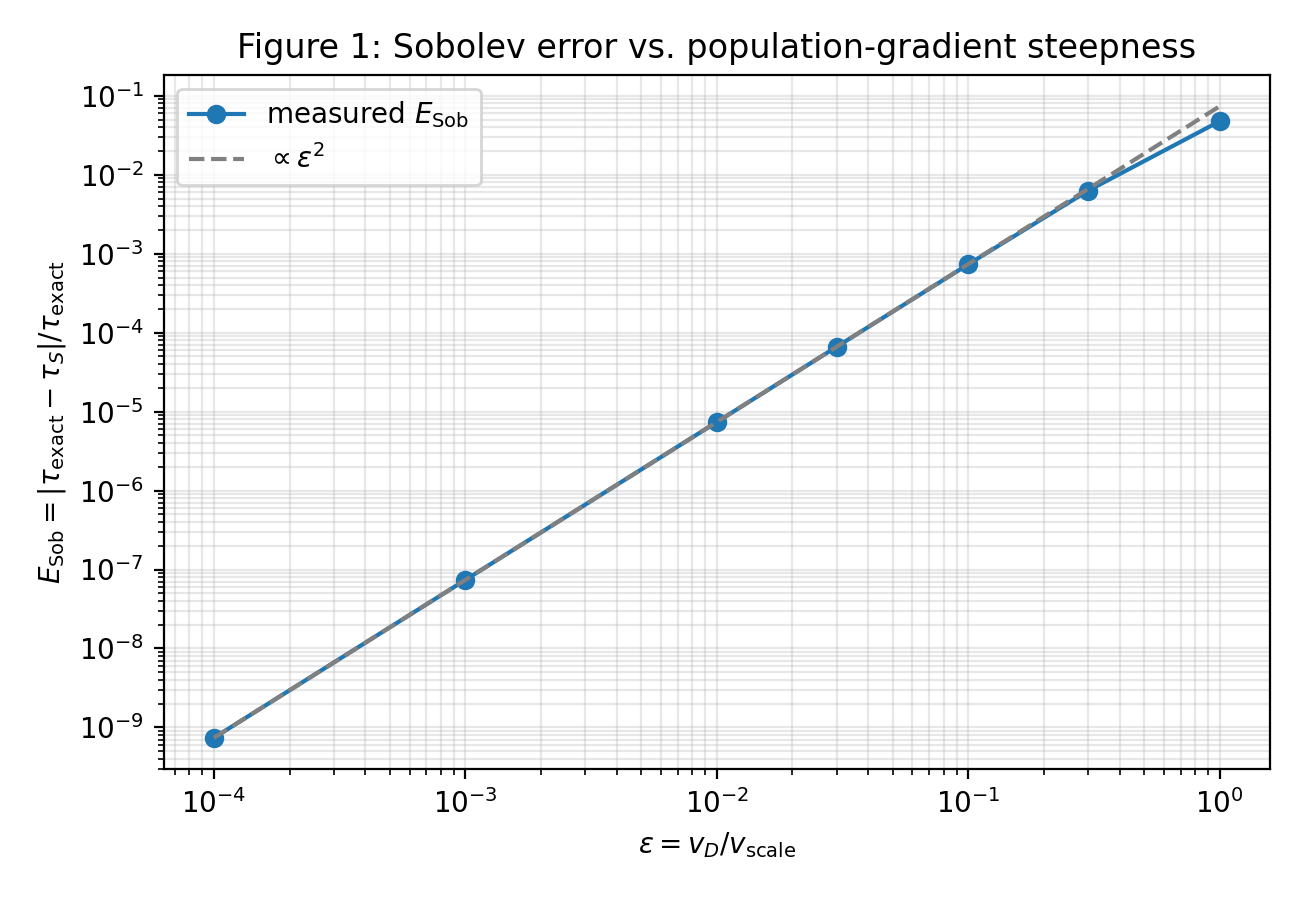
\includegraphics[width=0.78\textwidth]{fig1_sobolev_error_vs_gradient.png}
  \caption{Controlled breakdown of the Sobolev locality assumption. A
  $\tanh$-shaped population gradient of velocity scale $v_{\rm scale}$ is
  imposed; the relative error $E_{\rm Sob}$ between the resolved integral
  and the Sobolev formula follows the predicted $\epsilon^2$ power law in
  $\epsilon = v_D/v_{\rm scale}$ (measured log-slope 2.0000), reaching
  $\sim5\%$ when the gradient scale approaches the Doppler width.}
  \label{fig:grad}
\end{figure}

Before any code comparison, the toy problem: one line, constant $n_l$,
homologous slab. The resolved integral (Eq.~\ref{eq:tau}) converges to the
analytic $\taus$ (Eq.~\ref{eq:tausob}) to machine precision
($E_{\rm Sob}=2\times10^{-16}$ at $2\times10^{5}$ grid points), with
monotone convergence under refinement---important because an unconverged
grid mimics a physical Sobolev deviation.

Breaking locality on purpose (Fig.~\ref{fig:grad}) produced
\textbf{Finding F1}: with the population gradient placed \emph{symmetrically}
about the resonance point, the error cancels identically---the line profile
is even while the leading gradient term is odd, and the natural symmetric
choice ($\tanh$ centered on resonance) also has vanishing curvature there.
The error only appears when the resonance sits off-center on the gradient
(we use the point where curvature is large), and then follows a clean
$\epsilon^2$ law, at the few-percent level when
$\epsilon = v_D/v_{\rm scale} \gtrsim 0.3$
(Appendix~\ref{app:symmetry}). The practical consequence: widely used
validity diagnostics based on the gradient magnitude
$G = v_D\,|\mathrm{d}\ln n_l/\mathrm{d}v|$ are \emph{conservative}: the true
error depends on where the resonance sits on the gradient, and can be far
below the $G$-based bound.

\subsection{One line, three codes}

\begin{figure}[t]
  \centering
  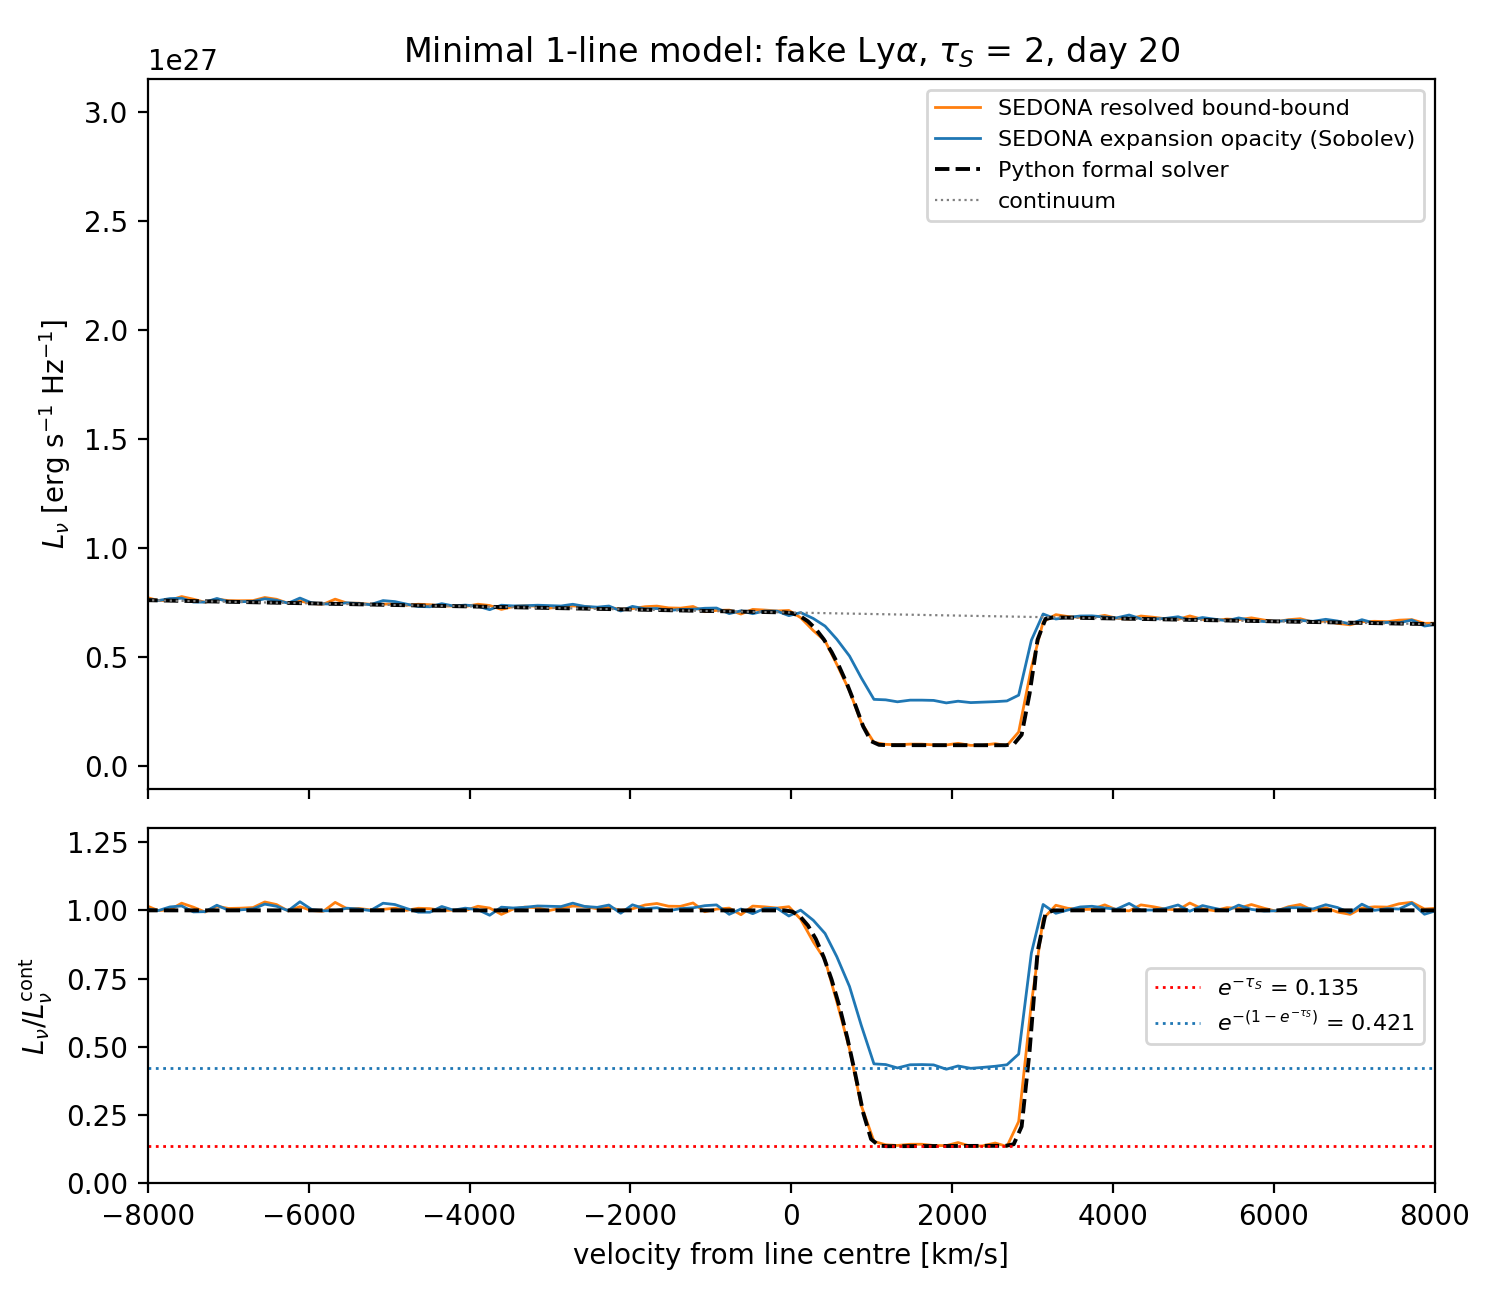
\includegraphics[width=0.85\textwidth]{fig4_minimal_1line_threeway.png}
  \caption{Minimal one-line model (artificial Ly$\alpha$-like line,
  $\taus=2$, cold neutral shell). Top: emergent spectra. Bottom: ratio to
  the continuum. \textsc{sedona}'s resolved mode (orange) lies on top of the
  deterministic solver (black dashed) across the entire profile, at the
  analytic depth $e^{-\taus}=0.135$ (red dotted). The expansion-opacity
  mode (blue) instead sits at the predicted capped value
  $e^{-(1-e^{-\taus})}=0.421$ (blue dotted).}
  \label{fig:minimal}
\end{figure}

The minimal cross-code experiment uses \textsc{sedona}'s built-in two-level
test atom (one line at 1215.5\,\AA, $f=0.665$) in a shell tuned to
$\taus=2$. The shell temperature (2000\,K) was chosen after an ionization-
balance check: at the very low densities that give $\taus\sim1$, a 5000\,K
gas would be fully ionized, destroying population control; at 2000\,K the
gas is neutral to one part in $10^{10}$.

The measured absorption-trough depths (Fig.~\ref{fig:minimal}):
\begin{center}
\begin{tabular}{@{}lc@{}}
\toprule
analytic $e^{-\taus}$ & 0.1353 \\
deterministic solver & 0.1372 \\
\textsc{sedona} resolved & 0.1420 \\
\textsc{sedona} expansion opacity & \textbf{0.4285} \\
predicted cap $e^{-(1-e^{-\taus})}$ & 0.4212 \\
\bottomrule
\end{tabular}
\end{center}

Two independent resolved implementations---deterministic rays and Monte
Carlo---agree with each other and with theory at the few-percent level
(\textbf{harness validated}), while the expansion-opacity mode lands within
$2\%$ of its own predicted cap, a factor $3.2$ too much transmitted light.
This is \textbf{Finding F4}: for a single strong line, ``Sobolev mode'' as
implemented via expansion opacity is \emph{not} Sobolev line transfer.

The same experiment surfaced \textbf{Finding F3}: the deterministic solver's
$1.4\%$ excess over the analytic value is exactly the
$\mathcal{O}(v_{\rm bulk}/c)$ frame ambiguity between observer-frame
integration and the comoving-frame Sobolev formula
(Appendix~\ref{app:frame}); at a resonance placed at $7.7\%$ of $c$ the
deviation grows to $7\%$ and matches $e^{-\taus(1-z_{\rm res}/ct)}$ to four
digits. All comparisons in this paper therefore keep resonances at
$v_{\rm bulk}/c < 1\%$; realistic-velocity comparisons will require matched
frame conventions.

\subsection{From two lines to a twenty-line ladder}

\begin{figure}[t]
  \centering
  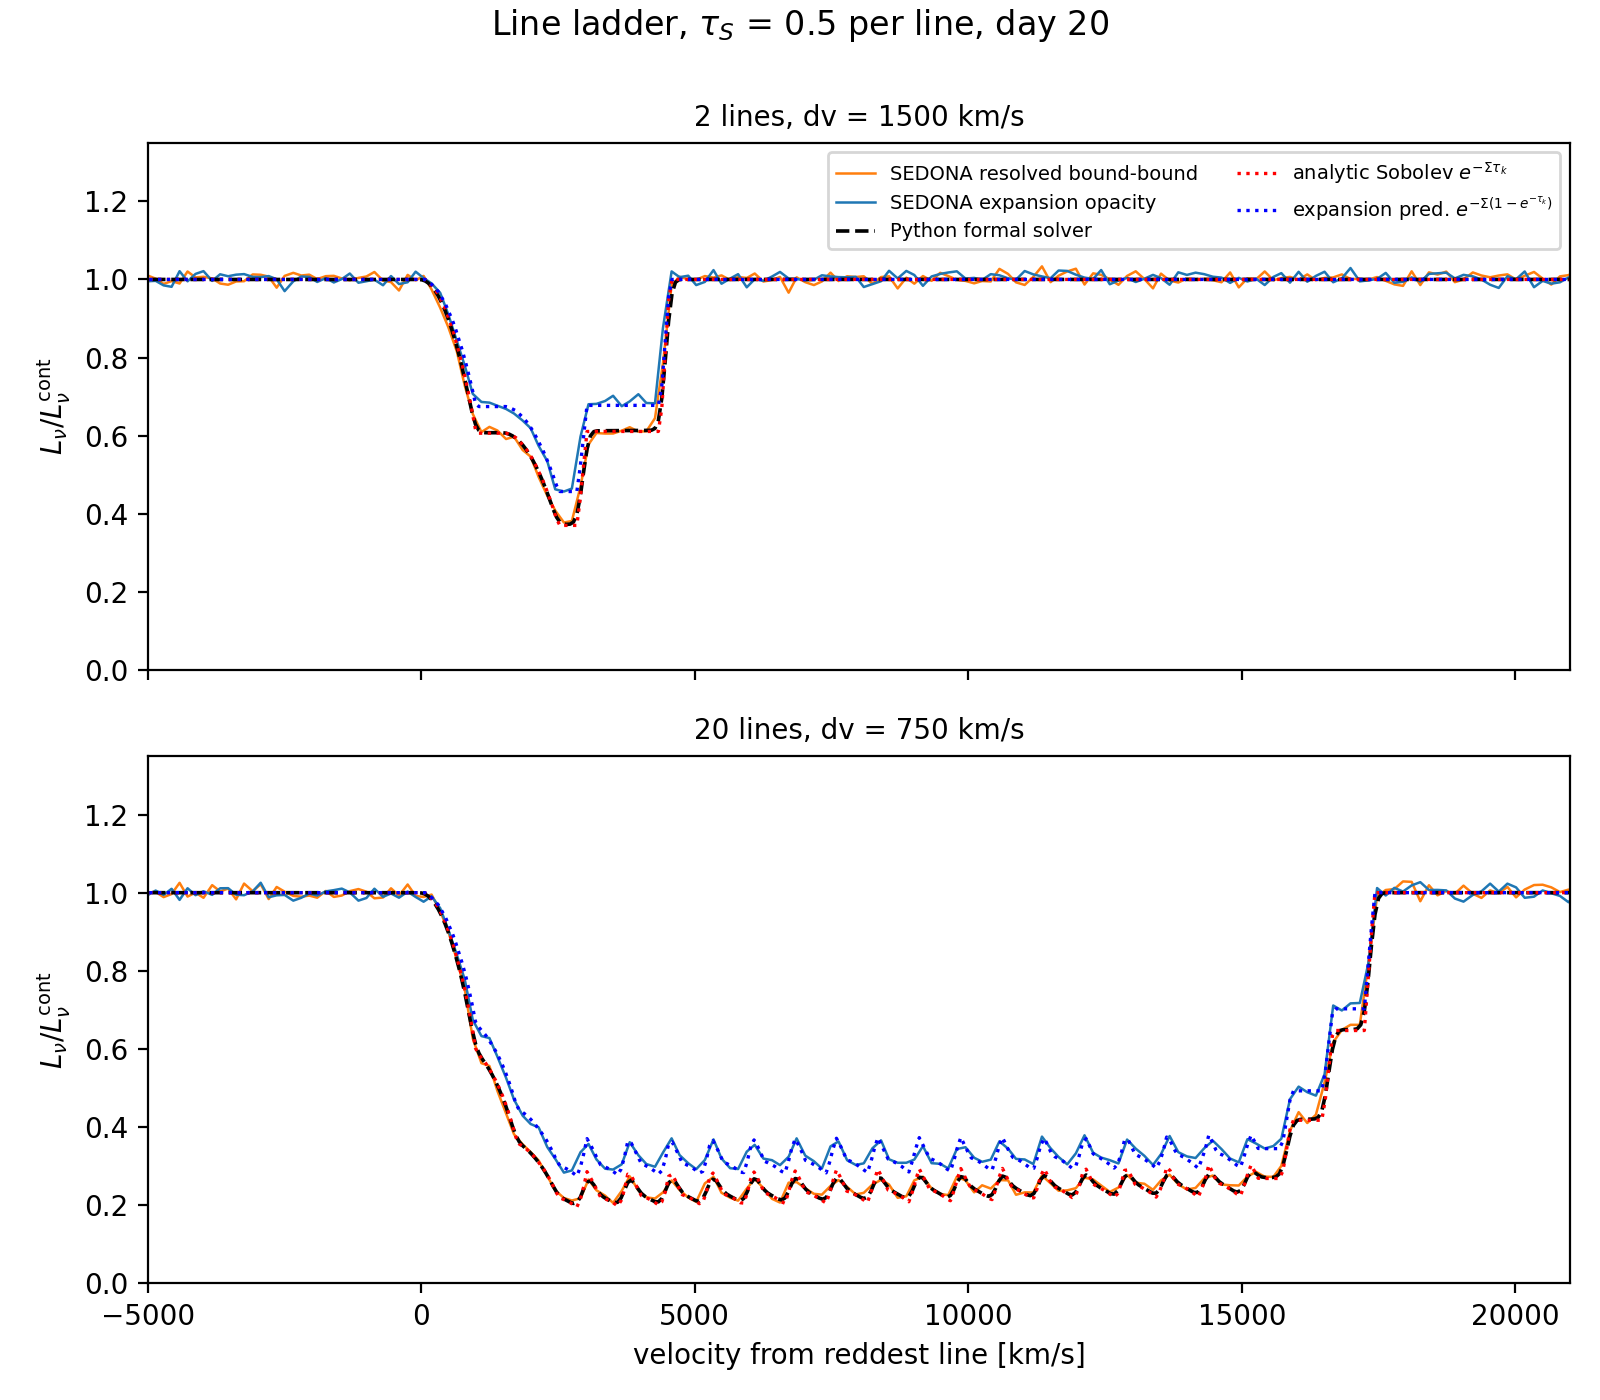
\includegraphics[width=0.9\textwidth]{fig5_line_ladder.png}
  \caption{Line ladder at $\taus = 0.5$ per line. Top: two lines separated
  by $1500\kms$ (overlapping troughs). Bottom: twenty lines spaced
  $750\kms$ (a mini forest). The resolved trio---\textsc{sedona} resolved
  (orange), deterministic solver (black dashed), $p$-averaged analytic
  staircase (red dotted)---lock together tooth for tooth; the expansion
  pair (blue solid: \textsc{sedona}; blue dotted: analytic cap prediction)
  ride systematically above them.}
  \label{fig:ladder}
\end{figure}

Custom \textsc{sedona} atomic files with 2 and then 20 identical-strength
lines ($\taus = 0.5$ each) test multi-line behavior
(Fig.~\ref{fig:ladder}). In the center of the 20-line forest, where each
photon crosses $\sim4$ resonances, five determinations of the transmitted
fraction give:
\begin{center}
\begin{tabular}{@{}lc@{}}
\toprule
analytic Sobolev ($p$-averaged) & 0.2405 \\
deterministic solver & 0.2407 \\
\textsc{sedona} resolved & 0.2435 \\
analytic expansion cap & 0.3194 \\
\textsc{sedona} expansion opacity & 0.3257 \\
\bottomrule
\end{tabular}
\end{center}

\textbf{Finding F5}: the expansion-opacity error tracks its own per-line
cap prediction, i.e.\ the error is incurred \emph{per resonance
crossing}. Adding more lines multiplies both the true and the capped
attenuations equally, so the fractional flux error does \emph{not} average
away with line count---it only vanishes as $\tau\to0$ per line. Expansion
opacity is a \emph{weak-line} approximation, not a many-line one.

A technical note that matters for anyone reproducing this: the analytic
staircase must be averaged over the stellar disk ($p$-average,
Appendix~\ref{app:pavg}), because resonance planes closer than the core
radius are crossed by only the outer rays; naive plane counting predicts
visibly too-shallow troughs.

%=====================================================================
\section{Results with real La II data}
\label{sec:results}

\subsection{Is the dangerous regime even populated? Line crowding}

\begin{figure}[t]
  \centering
  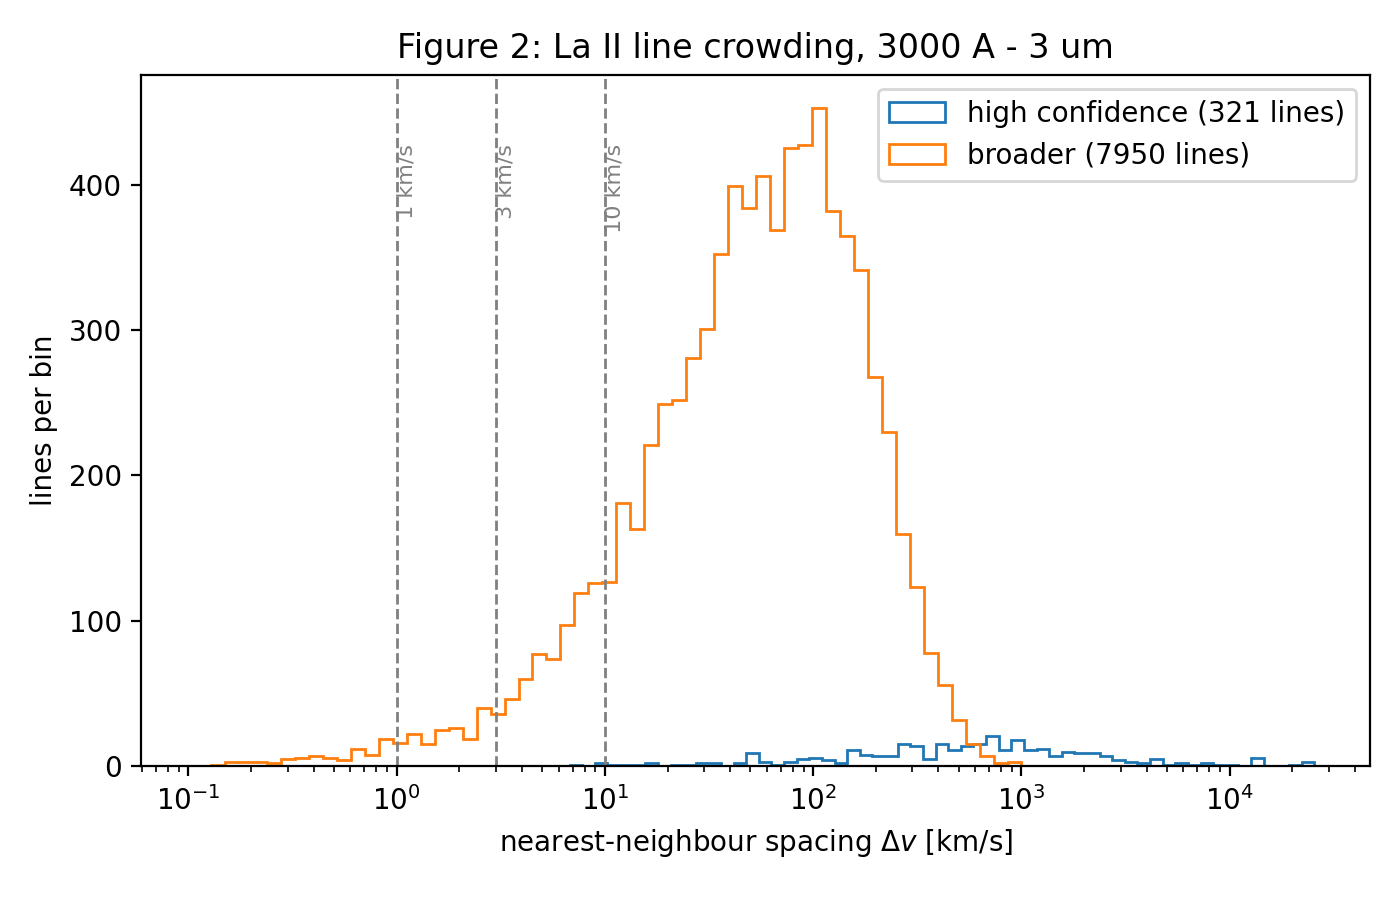
\includegraphics[width=0.8\textwidth]{fig2_laII_line_spacing.png}
  \caption{Nearest-neighbor velocity spacing of GSI La\,\textsc{ii} lines
  (3000\,\AA--3\,$\mu$m): in the broader subset, $11.3\%$ of lines have a
  neighbor within $10\kms$ and $3.3\%$ within $3\kms$.}
  \label{fig:crowding}
\end{figure}

The Sobolev isolation assumption fails when lines crowd within a Doppler
width. Fig.~\ref{fig:crowding} shows that even for this \emph{single} ion,
the calibrated data contain a real crowding tail: $11.3\%$ of the broader
line sample has a neighbor within $10\kms$. Multi-ion mixtures only add
lines, so the potentially problematic regime exists in nature.

\subsection{A realistic forest: 153 calibrated lines}

\begin{figure}[t]
  \centering
  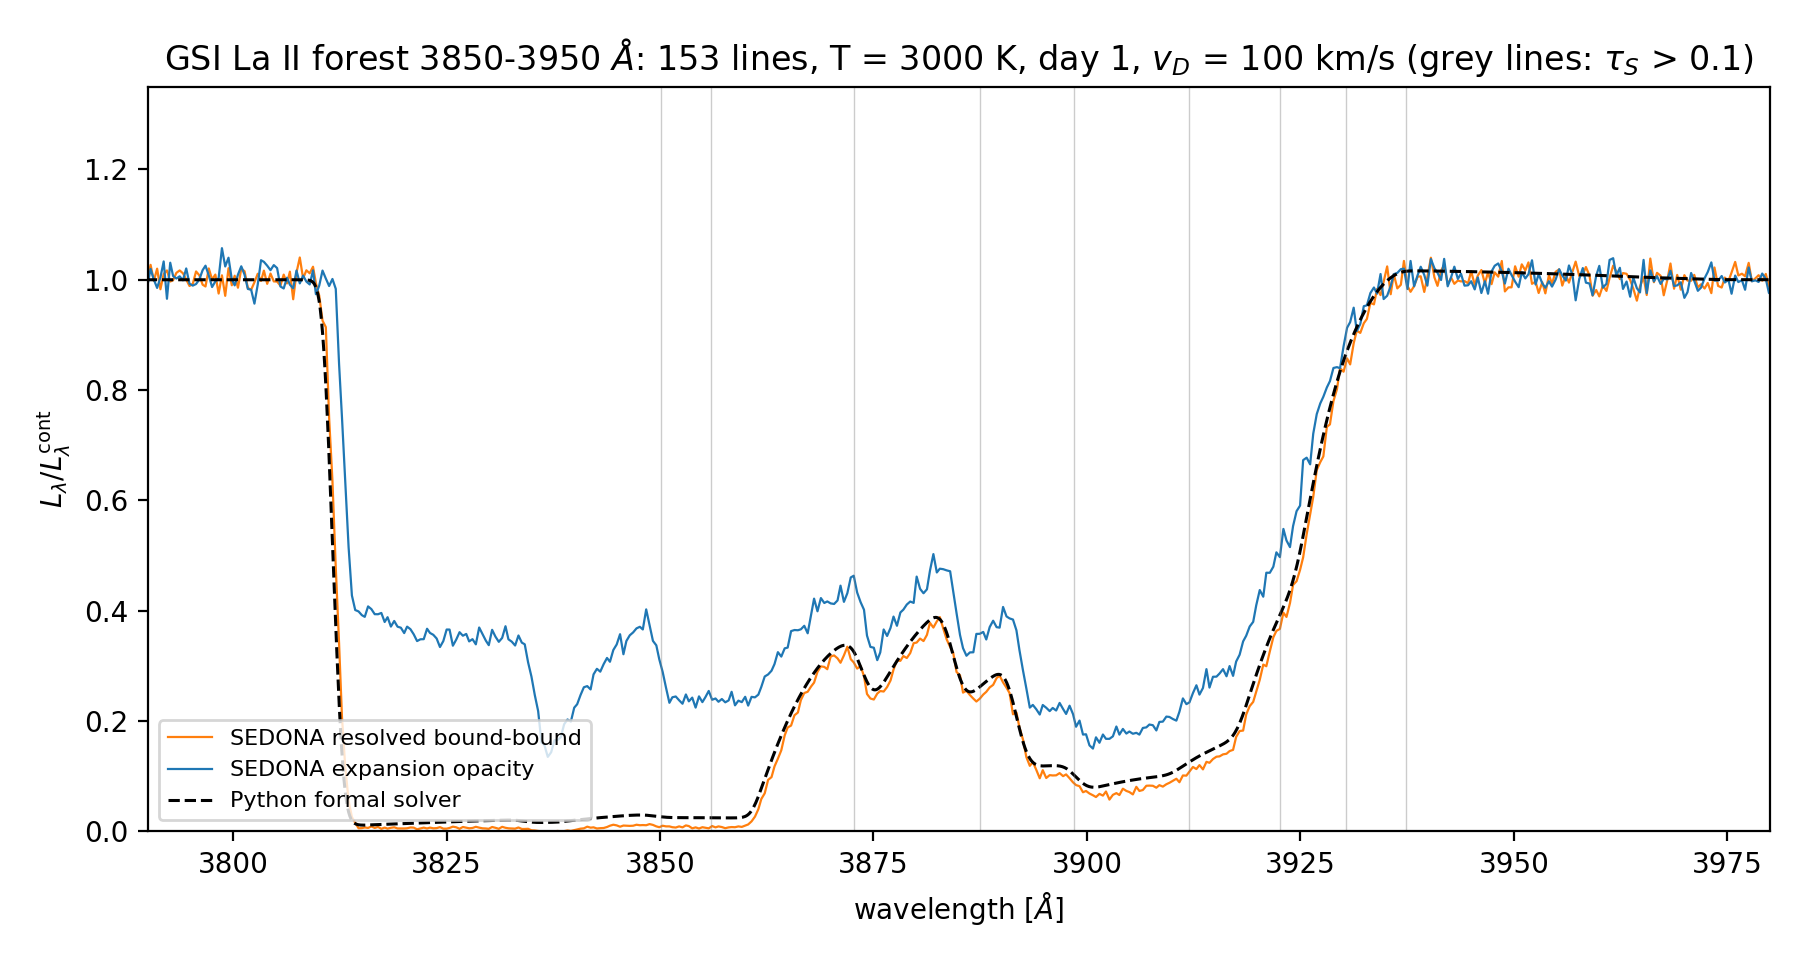
\includegraphics[width=\textwidth]{fig6_laII_forest.png}
  \caption{The 3850--3950\,\AA{} La\,\textsc{ii} forest (153 calibrated
  lines, 3 with $\taus>1$, max 5) at $T=3000$\,K, one day after merger.
  The resolved treatments (orange, black dashed) saturate to black where
  strong troughs overlap; expansion opacity (blue) never drops below
  $\sim0.2$ because each crossing is capped.}
  \label{fig:forest}
\end{figure}

We select the 100\,\AA{} window with the richest optical-depth distribution
(3850--3950\,\AA), build the population-controlled \textsc{sedona} atom from
the GSI data (Section~\ref{sec:popcontrol}), and run the three-way
comparison at $T = 3000$\,K, $t = 1$\,day, Doppler width $100\kms$
(Fig.~\ref{fig:forest}). Band-averaged transmitted flux over
3800--3955\,\AA:
\begin{center}
\begin{tabular}{@{}lc@{}}
\toprule
deterministic solver & 0.3549 \\
\textsc{sedona} resolved & 0.3426 \\
\textsc{sedona} expansion opacity & 0.4965 \\
\midrule
$\dsob$ & $\mathbf{+44.9\%}$ \\
\bottomrule
\end{tabular}
\end{center}

The resolved pair agree to $3.6\%$ as tabulated---and to $1.0\%$ once the
thermal-emission convention is matched (Finding F8,
\S\ref{sec:conventions-f8})---while the expansion-opacity run overestimates
the transmitted band flux by $45\%$. Notably this exceeds the uniform-ladder
error ($+35\%$ at $\tau=0.5$ per line): real forests are dominated by a few
strong lines, precisely where the per-crossing cap is most wrong.

\subsection{The validity map: strength, width, temperature}

\begin{figure}[t]
  \centering
  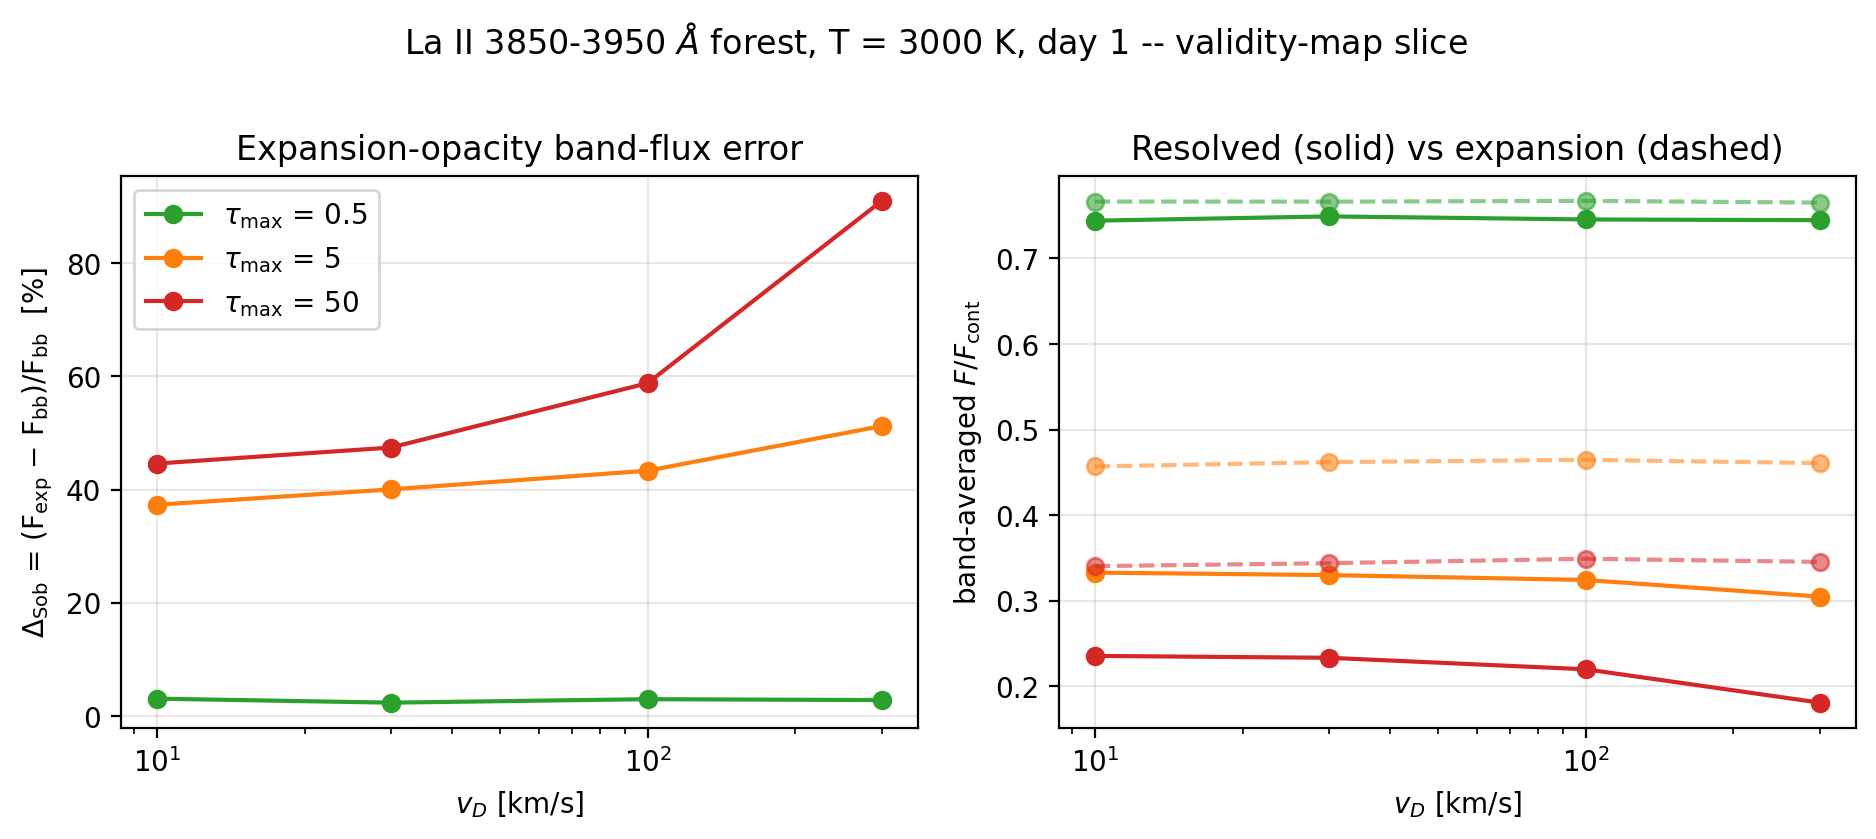
\includegraphics[width=\textwidth]{fig7_validity_slice.png}
  \caption{First validity-map slice: $\dsob$ vs Doppler width for three
  overall line-strength scalings of the La\,\textsc{ii} forest. Right
  panel: expansion-opacity fluxes (dashed) are blind to $v_D$, while
  resolved fluxes (solid) drop as profiles widen.}
  \label{fig:slice}
\end{figure}

\begin{figure}[t]
  \centering
  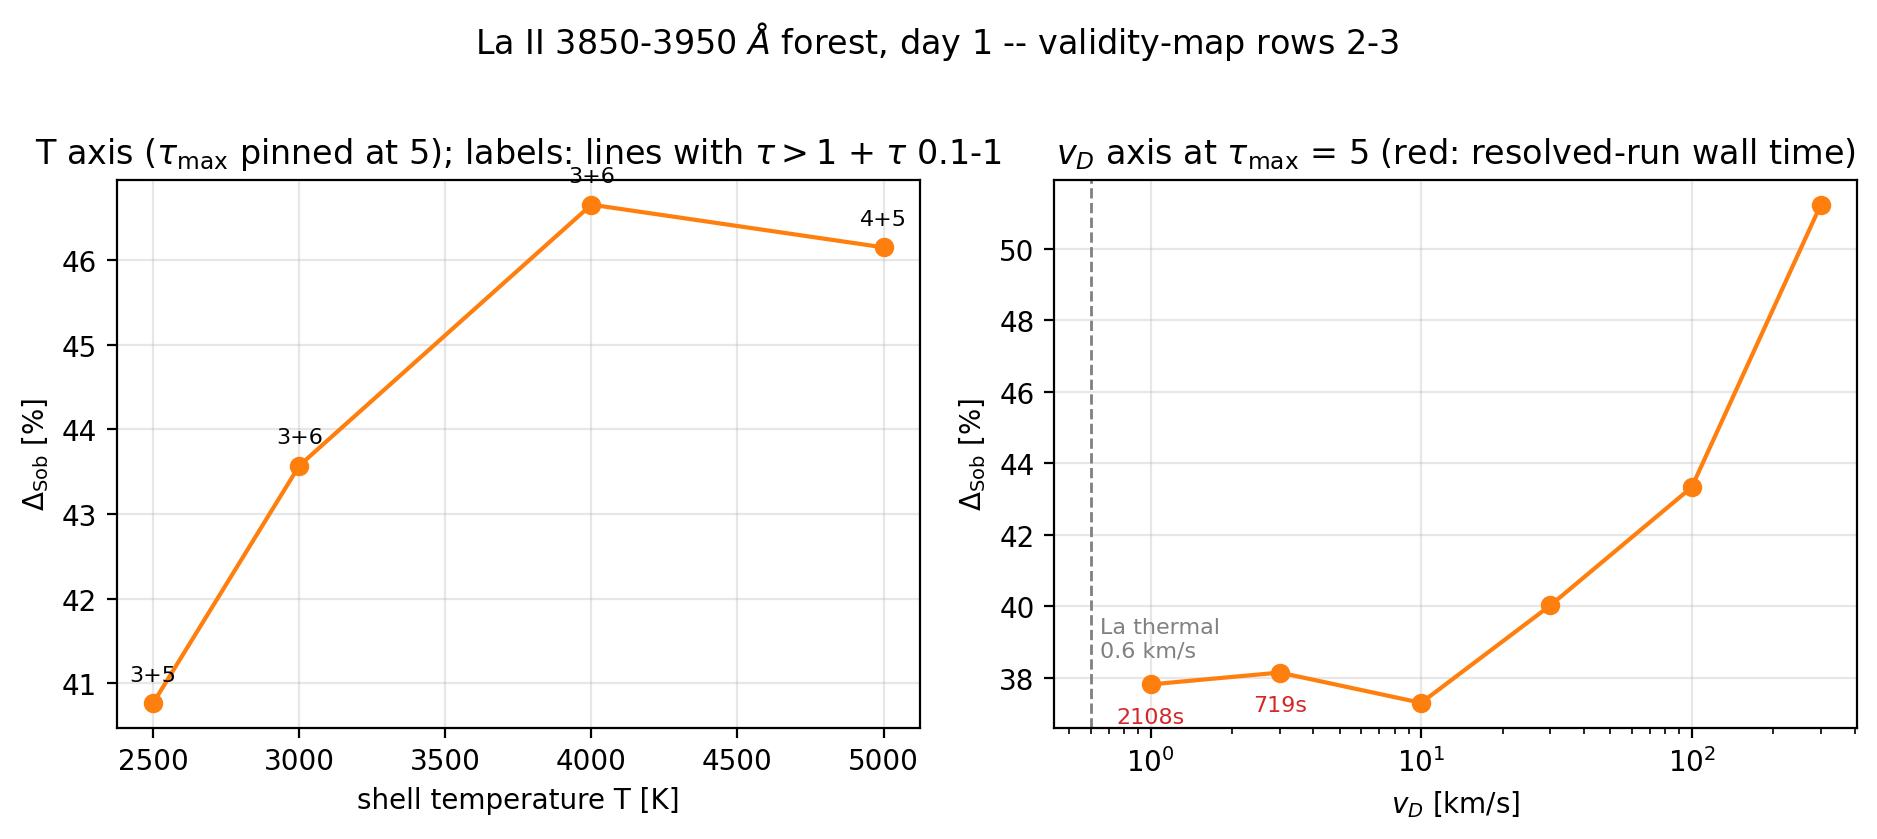
\includegraphics[width=\textwidth]{fig8_T_and_frontier.png}
  \caption{Left: temperature axis at pinned $\tau_{\max}=5$ (weak
  dependence; annotations count strong lines). Right: the Doppler-width
  frontier: $\dsob$ is flat at $\sim38\%$ from $10\kms$ down to $1\kms$,
  essentially the La thermal width; red annotations give the resolved-run
  wall time.}
  \label{fig:frontier}
\end{figure}

Scaling the overall line strength ($\tau_{\max}\in\{0.5,5,50\}$ by scaling
the ion density) and the Doppler width
($v_D \in \{1,3,10,30,100,300\}\kms$) yields the first rows of the validity
map (Figs.~\ref{fig:slice}--\ref{fig:frontier}; $\dsob$ in percent):

\begin{center}
\begin{tabular}{@{}lcccccc@{}}
\toprule
$\tau_{\max}\backslash v_D$ & 1 & 3 & 10 & 30 & 100 & 300 km/s\\
\midrule
0.5 & -- & -- & $+3.0$ & $+2.3$ & $+2.9$ & $+2.8$ \\
5   & $+37.8$ & $+38.1$ & $+37.3$ & $+40.0$ & $+43.3$ & $+51.2$ \\
50  & -- & -- & $+44.6$ & $+47.4$ & $+58.8$ & $+91.1$ \\
\bottomrule
\end{tabular}
\end{center}

\textbf{Finding F6}: the error decomposes into
\begin{enumerate}
  \item a \emph{strength-set floor}, independent of $v_D$: the pure
  per-crossing substitution error. Weak forests are safe at the $3\%$
  level; by $\tau_{\max}=5$ the floor is $\sim38\%$;
  \item a \emph{wing term} growing with $v_D$: expansion opacity is
  width-blind (its transmitted flux is flat across a factor 300 in $v_D$),
  while genuinely wide lines absorb continuum between resonances.
\end{enumerate}
The frontier measurement at $1\kms$---within a factor 2 of the actual
La thermal width---confirms that the floor survives: \emph{no refinement of
line widths rehabilitates expansion opacity in the strong-line regime}.

The temperature axis (Fig.~\ref{fig:frontier}, left), with strength pinned,
moves $\dsob$ only from $+41\%$ to $+47\%$ across 2500--5000\,K: in this
window the same few strong lines dominate at all temperatures, so
population redistribution is a weak axis (single-ion result; multi-ion
mixtures may differ).

\subsection{Multi-ion blending and the density dependence}
\label{sec:multiion}

\begin{figure}[t]
  \centering
  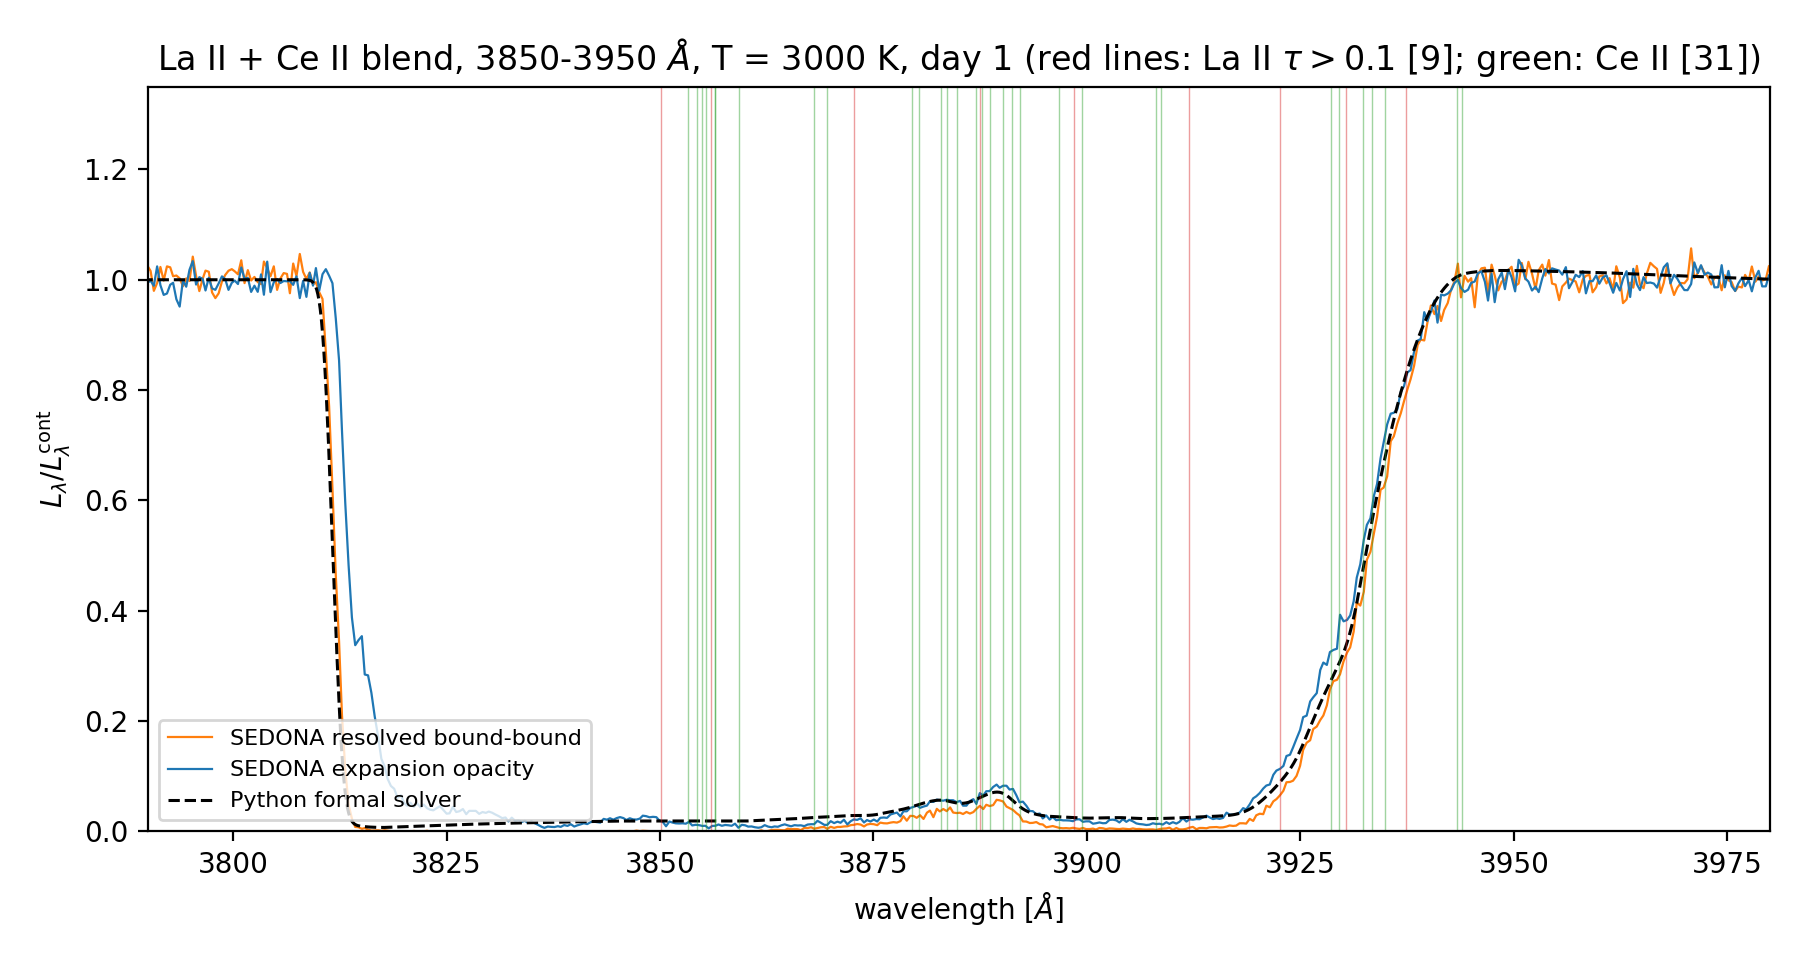
\includegraphics[width=\textwidth]{fig9_multiion_forest.png}
  \caption{La\,\textsc{ii} + Ce\,\textsc{ii} blend in the same window. Ce
  floods it with 2376 additional lines (2529 total; strong-line spacings
  down to $8\kms$), saturating the band to near-black in every treatment.}
  \label{fig:blend}
\end{figure}

Adding Ce\,\textsc{ii} at equal mass fraction multiplies the line count by
$16$ and drives strong-line separations down to $8\kms$---genuine
sub-Doppler blending. The measured error, however, \emph{falls}, to
$\dsob = +14.6\%$ (Fig.~\ref{fig:blend}).

\textbf{Finding F7}: $\dsob$ is non-monotonic in forest density. With enough
crossings, even capped per-crossing contributions sum to blackness, so both
treatments agree that almost nothing escapes and the relative error is
suppressed. The regime that maximizes the error is the \emph{intermediate}
one---strong lines that do not yet fully blanket the band---which is exactly
where spectral features form and where composition is read off.

\subsection{Which approximation is at fault? Separating the two errors}
\label{sec:separation}

\begin{figure}[t]
  \centering
  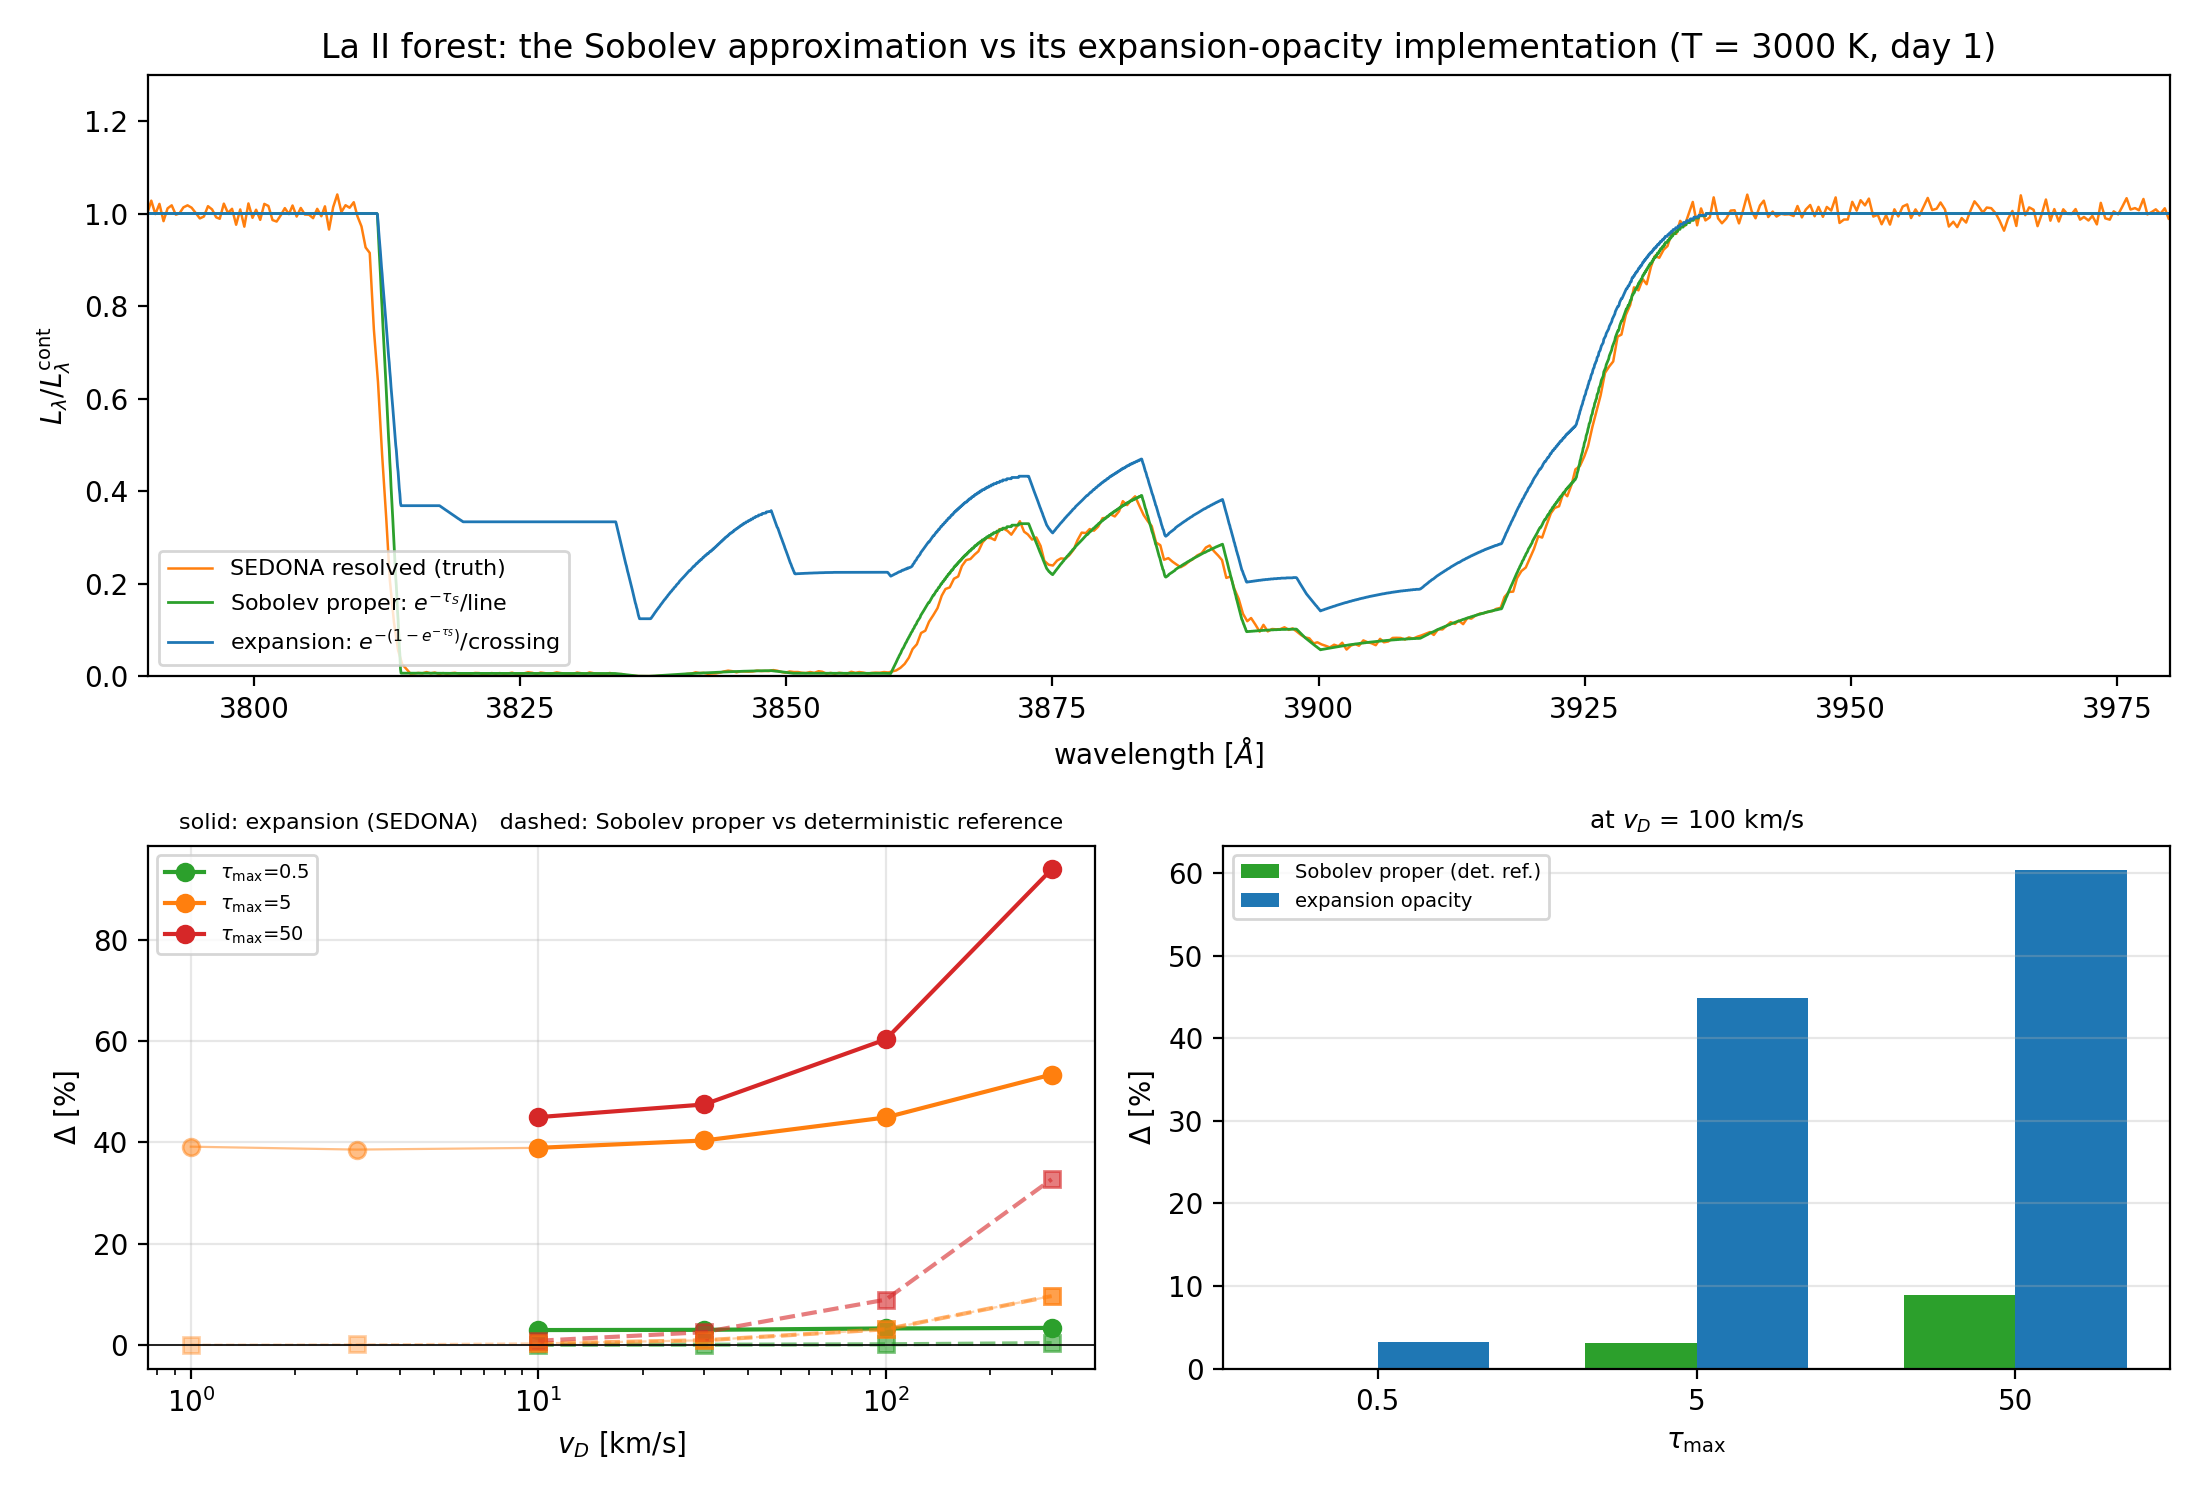
\includegraphics[width=\textwidth]{fig10_sobolev_vs_expansion.png}
  \caption{Top: the La\,\textsc{ii} forest under three treatments. The
  Sobolev approximation proper (green, per-line $e^{-\taus}$) tracks the
  resolved calculation (orange) closely; expansion opacity (blue) sits well
  above it. Bottom left: both errors versus Doppler width, for three
  line-strength scalings (solid: expansion; dashed: Sobolev). Bottom right:
  the two at $v_D = 100\kms$.}
  \label{fig:separation}
\end{figure}

Everything above measures the expansion-opacity \emph{implementation}. We now
measure the Sobolev approximation \emph{itself}---per-line $e^{-\taus}$ with
delta-function resonances---against the same truth. In this pure-absorption
LTE configuration that prediction is exact analytics (the $p$-averaged
staircase of Appendix~\ref{app:pavg}), so no additional transport
calculations are required; the identical machinery yields the expansion
prediction by damping each crossing with $1-e^{-\tau}$.

For the La\,\textsc{ii} forest, against \textsc{sedona} resolved $=0.3426$:
Sobolev proper gives $0.3507$ ($+2.4\%$) while expansion opacity gives
$0.4965$ ($+44.9\%$). Across the sweep (Fig.~\ref{fig:separation}):

\begin{center}
\begin{tabular}{@{}cccc@{}}
\toprule
$\tau_{\max}$ & $v_D$ [km/s] & $\Delta$ Sobolev & $\Delta$ expansion \\
\midrule
0.5 & 10  & $+7.1\%$ & $+3.0\%$ \\
0.5 & 300 & $+7.0\%$ & $+2.8\%$ \\
5   & 10  & $+5.4\%$ & $+37.3\%$ \\
5   & 300 & $+15.1\%$ & $+51.2\%$ \\
50  & 10  & $+7.1\%$ & $+44.6\%$ \\
50  & 300 & $+39.4\%$ & $+91.1\%$ \\
\bottomrule
\end{tabular}
\end{center}

\textbf{Finding F9}: the two components of F6 have different owners.
\emph{The strength-set floor belongs to expansion opacity alone.} Sobolev
proper exhibits no strength floor at all---it is $+5$--$7\%$ at
$\tau_{\max}=0.5$, $5$ and $50$ alike at small $v_D$---while expansion climbs
$+3\% \to +37\% \to +45\%$. That floor is the per-crossing cap, not a failure
of locality or isolation. \emph{The width-growing term, by contrast, is a
genuine Sobolev failure}: a delta-function resonance has no width by
construction, so the Sobolev leg is exactly $v_D$-independent and all of the
resolved calculation's width dependence is unmodelled, reaching $+39\%$ at
$(\tau_{\max}, v_D) = (50, 300\kms)$.

The headline is therefore sharper than either treatment alone suggests: at
kilonova-relevant line widths ($\lesssim 30\kms$) \textbf{the Sobolev
approximation is accurate to $\approx 5$--$8\%$, while its standard
expansion-opacity implementation errs by $40$--$90\%$}. The literature
conflates the two under one name; they are different approximations and they
fail for different reasons.

Two caveats. At $\tau_{\max}=0.5$ the \textsc{sedona} expansion result
($+3.0\%$) is closer to truth than Sobolev proper ($+7.1\%$), but this is
compensating error rather than accuracy: the analytic cap there is $+10.1\%$,
and \textsc{sedona}'s binning smears absorption into inter-line gaps,
darkening the spectrum by $\sim6\%$ and offsetting the cap's
over-transmission. And the residual $+5$--$7\%$ Sobolev floor at small $v_D$
is not explained by line strength; the natural candidate is overlap within a
Doppler width---the isolation assumption---which the crowding statistics of
\S\ref{sec:results} show is present in these data.

\subsection{A convention that must be matched: thermal emission}
\label{sec:conventions-f8}

\textbf{Finding F8}, recorded because it is a trap for anyone benchmarking a
deterministic solver against a Monte Carlo code. Our solver integrates the
LTE source term $S_\nu = B_\nu(T_{\rm shell})$ along every ray;
\textsc{sedona}, run at fixed temperature with radiative equilibrium
disabled, deposits absorbed packet energy without re-emitting it. Setting
$T_{\rm shell}\to0$ in the solver isolates the difference exactly: the
single-ion forest moves $0.3538 \to 0.3390$ against \textsc{sedona}'s
$0.3426$ ($+3.3\% \to -1.0\%$), and the blend $0.2410 \to 0.2249$ against
$0.2277$ ($+6.5\% \to -1.2\%$). Like for like, the two independent codes
agree at the $\sim1\%$ Monte Carlo noise floor. The term exceeds the naive
$B_\nu(3000)/B_\nu(6000) = 2\times10^{-3}$ estimate because the shell
subtends nine times the core's projected area, and it grows with saturation.
Absolute band fluxes quoted from \textsc{sedona} in this configuration are
therefore attenuation-only; $\dsob$, a differential between two
\textsc{sedona} runs sharing one convention, is unaffected.

\subsection{Computational cost}

\begin{figure}[t]
  \centering
  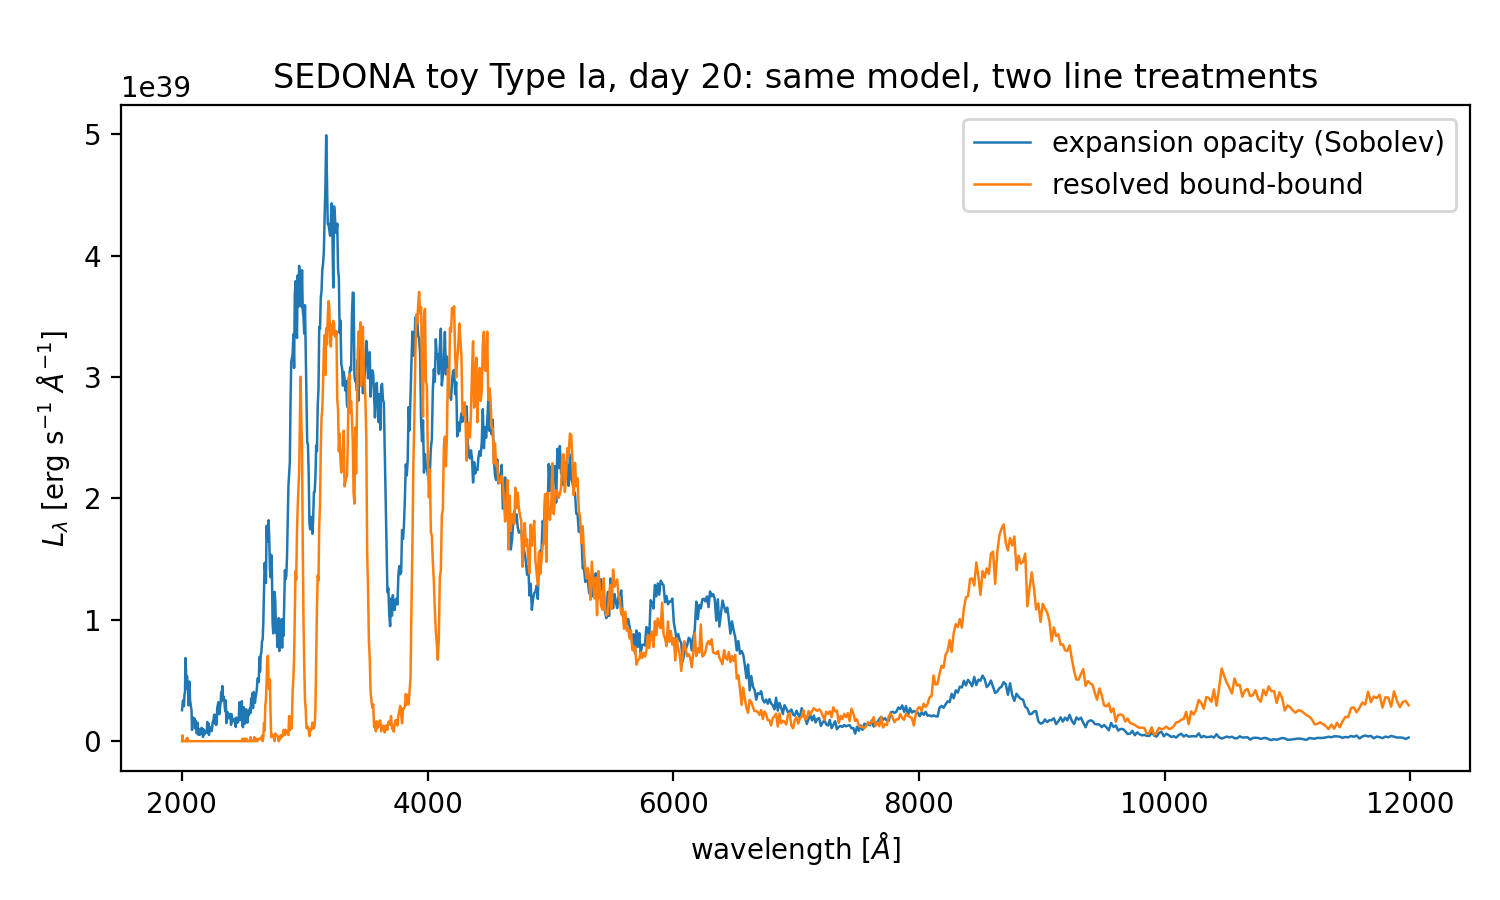
\includegraphics[width=0.9\textwidth]{fig3_sedona_typeIa_exp_vs_bb.png}
  \caption{Motivating cost anecdote from a standard \textsc{sedona}
  Type~Ia supernova example: the same model runs in 14\,s with expansion
  opacity and 88\,min resolved ($378\times$), while redistributing flux
  from the UV to the near-IR.}
  \label{fig:cost}
\end{figure}

Why does everyone use the shortcut? Cost. On a standard \textsc{sedona}
Type~Ia example, switching from expansion opacity to the resolved treatment
multiplied the run time by $378$ (Fig.~\ref{fig:cost}). Our sweep adds a
cleaner measurement: in the controlled forest, resolved-run wall time scales
as $1/v_D$ (25\,s at $100\kms$, 719\,s at $3\kms$, 2109\,s at $1\kms$),
driven entirely by the transport frequency grid---and the expansion run on
the same fine grid costs the same (2305\,s at $1\kms$). The expense is the
grid, not the physics; narrow windows keep resolved calculations
affordable, which is the strategy this program uses.

%=====================================================================
\section{Discussion}
\label{sec:discussion}

\begin{table}[t]
\centering
\caption{Findings register.}
\label{tab:findings}
\begin{tabular}{@{}clc@{}}
\toprule
\# & Finding & Where \\
\midrule
F1 & Symmetric gradients cancel the Sobolev error at leading order; & \S\ref{sec:verification} \\
   & gradient-based diagnostics are conservative & \\
F2 & Resolved vs expansion cost: $378\times$ on a standard example & \S\ref{sec:results} \\
F3 & $\mathcal{O}(v_{\rm bulk}/c)$ frame ambiguity between observer-frame & \S\ref{sec:verification} \\
   & integration and comoving Sobolev $\tau$ & \\
F4 & Expansion opacity transmits $e^{-(1-e^{-\tau})}$ per crossing, not $e^{-\tau}$ & \S\ref{sec:verification} \\
F5 & That error is per-resonance: it does not average away with line count & \S\ref{sec:verification} \\
F6 & $\dsob$ = strength-set floor + $v_D$-growing wing term; & \S\ref{sec:results} \\
   & the floor survives to thermal widths & \\
F7 & $\dsob$ is non-monotonic in forest density: maximal for strong & \S\ref{sec:multiion} \\
   & sparse forests, suppressed at full line blanketing & \\
F8 & Solver-vs-MC offsets trace to the thermal-emission convention, & \S\ref{sec:conventions-f8} \\
   & not to profiles or resolution; matched, the codes agree to $\sim1\%$ & \\
F9 & The strength floor is expansion opacity's alone; the width term & \S\ref{sec:separation} \\
   & is a genuine Sobolev failure. Sobolev $\approx5$--$8\%$ vs $40$--$90\%$ & \\
\bottomrule
\end{tabular}
\end{table}

\paragraph{What the floor means for kilonova modeling.}
Lanthanide-rich ejecta are the definition of the strong-line regime: Sobolev
depths of important lines reach $10^{2}$--$10^{4}$ in the line-forming
region. Our measurements say that in that regime the expansion-opacity
treatment overestimates band-integrated transmitted flux by tens of percent
\emph{as a floor}, independent of how finely line profiles are treated. Band
fluxes feed directly into inferred ejecta masses and compositions; a
systematic of this size and sign (too much blue light escaping) plausibly
biases lanthanide-fraction inferences. Quantifying that propagation to
observables is future work.

\paragraph{Which approximation did we actually test?}
An important distinction this study sharpens: the error measured here is
that of the \emph{expansion-opacity implementation} of the Sobolev idea---
the standard choice in multi-group Monte Carlo codes---and not of a
per-line Sobolev interaction scheme (as implemented in, e.g., TARDIS-class
codes), which applies $e^{-\taus}$ per line and would not exhibit the
per-crossing cap (F4/F5). The two are routinely conflated under the name
``Sobolev approximation.'' A per-line Sobolev leg in this harness is
planned; the genuinely Sobolev-intrinsic errors (locality F1, overlap
within a Doppler width) are bounded here by the resolved-vs-analytic
agreements and appear far smaller than the expansion-opacity cap in all
regimes probed so far.

\paragraph{Limitations.}
Pure absorption with LTE populations (no scattering, fluorescence, or
NLTE); fixed temperatures; controlled shell velocities
($1000$--$3000\kms$) rather than realistic $0.1$--$0.3c$ (pending
frame-consistent treatment, F3); Doppler widths down to $1\kms$ but not the
$0.6\kms$ thermal value; one ion, one window, one epoch so far; Monte Carlo
noise $\sim1$--$2\%$ per band flux. None of these caveats touches the sign
or order of magnitude of the central result, which is reproduced
independently by analytic theory (Appendix~\ref{app:expop}).

%=====================================================================
\section{Conclusions and next steps}

We built and validated a three-way harness that isolates the line-transfer
treatment in expanding ejecta, and used it to make the first controlled
measurements of the expansion-opacity error on calibrated lanthanide data.
The headline: the error has a floor set by line strength alone ($\sim38\%$
in band flux for a realistic La\,\textsc{ii} forest with $\tau_{\max}=5$)
that survives to thermal line widths. In the strong-line regime that
kilonovae occupy, ``Sobolev mode'' as commonly implemented is a
weak-line approximation being used outside its domain.

Next: multi-ion forests (Ce\,\textsc{ii}/\textsc{iii} from the same
database), additional windows and epochs, a per-line Sobolev leg to
separate approximation from implementation, and frame-consistent
comparisons at realistic velocities.

\section*{Reproducibility}

All code, data provenance, executed notebooks, experiment generators, and
this manuscript live at
\url{https://github.com/zhuygln/revisit_sobolev}. Atomic data: GSI Database
for Kilonova Radiative Transfer, Zenodo record 19335084 (CC-BY 4.0).
Radiative transfer: the public \textsc{sedona} release
(\url{https://github.com/dnkasen/pubsed}). Every figure regenerates from a
committed script; the 19-test suite pins the physics of every module.

%=====================================================================
\appendix

\section{Derivations for the non-specialist}

\subsection{The formal solution and thermal populations}
\label{app:formal}

Multiply Eq.~(\ref{eq:rte}) by $e^{\tau}$ with
$\mathrm{d}\tau = \alpha\,\mathrm{d}s$ and integrate: the intensity leaving
a slab is
\begin{equation}
  I^{\rm out}
  = I^{\rm in} e^{-\tau_{\rm tot}}
  + \int_0^{\tau_{\rm tot}} S(\tau')\, e^{-(\tau_{\rm tot}-\tau')}\,
  \mathrm{d}\tau',
  \qquad S \equiv j/\alpha .
  \label{eq:formalsol}
\end{equation}
The first term is the attenuated input beam; the second adds the gas's own
emission, each parcel attenuated by the material still in front of it. The
deterministic solver evaluates Eq.~(\ref{eq:formalsol}) numerically along
each ray with $S = B_\nu(T)$, accumulating $\tau$ by the trapezoidal rule;
convergence requires resolving the Doppler width along the path.

In thermal equilibrium the fraction of ions in level $i$ (energy $E_i$,
statistical weight $g_i = 2J_i+1$) is
\begin{equation}
  \frac{n_i}{n_{\rm ion}}
  = \frac{g_i\, e^{-E_i/k_BT}}{\sum_j g_j\, e^{-E_j/k_BT}} .
\end{equation}
A subtlety our tests caught: the \emph{fraction per statistical weight} is
what decreases monotonically with energy; raw fractions need not (at
3000--5000\,K a $g=7$ level at 1016\,cm$^{-1}$ out-populates the $g=5$
ground state of La\,\textsc{ii}).

\subsection{The Sobolev optical depth}
\label{app:sobolev}

Along a ray toward the observer, the gas at coordinate $z$ moves with
line-of-sight velocity $z/t$ (homologous flow), so a photon of observer
frequency $\nu$ has gas-frame frequency
$\nu' = \nu\,(1 - z/ct)$ to first order in $v/c$. Insert the line opacity
(Eq.~\ref{eq:linealpha}) into the optical-depth integral
(Eq.~\ref{eq:tau}) and change variables from $z$ to $\nu'$
($\mathrm{d}\nu' = -(\nu/ct)\,\mathrm{d}z \approx -(\nu_0/ct)\,\mathrm{d}z$
near resonance):
\begin{equation}
  \tau
  = \sigma_{\rm cl} f \int n_l(z)\, \phi(\nu'-\nu_0)\, \mathrm{d}z
  \;\approx\;
  \sigma_{\rm cl} f\, n_l(z_{\rm res})\, \frac{ct}{\nu_0}
  \underbrace{\int \phi\, \mathrm{d}\nu'}_{=1}
  = \sigma_{\rm cl} f\, n_l\, \lambda_0\, t ,
\end{equation}
which is Eq.~(\ref{eq:tausob}). The two approximations made are exactly the
two Sobolev assumptions: $n_l$ was pulled out of the integral at its
resonance-point value (locality), and the profile was integrated as if no
other line interfered (isolation).

\subsection{Why a symmetric gradient cancels (F1)}
\label{app:symmetry}

Let $n_l(v) = n_0[1 + g(v - v_{\rm res})]$ with $g$ odd about the resonance
(e.g.\ $\tanh$ centered there). The resolved integral weights $n_l$ by the
even profile $\phi$; the odd term integrates to zero, so the first-order
error vanishes. The next term is set by the curvature
$n_l''(v_{\rm res})$---which for a centered $\tanh$ \emph{also} vanishes
(inflection point). Only with the resonance off-center does the curvature
term survive, giving
$E_{\rm Sob} \simeq \tfrac12 |n_l''/n_l|\, \sigma_v^2 \propto \epsilon^2$,
the law measured in Fig.~\ref{fig:grad}.

\subsection{The expansion-opacity cap (F4)}
\label{app:expop}

Integrate the binned opacity of Eq.~(\ref{eq:expop}) along the stretch of
path over which the moving gas keeps one line inside one frequency bin.
The Doppler sweep rate ties path length to bin width,
$\Delta z = ct\,\Delta\nu_{\rm bin}/\nu$, so the effective optical depth
contributed by line $k$ is
\begin{equation}
  \tau^{\rm eff}_k
  = \alpha^{\rm exp}\,\Delta z
  = \frac{1}{ct}\,\frac{\nu_k}{\Delta\nu_{\rm bin}}
    \left(1-e^{-\tau_{{\rm S},k}}\right)\times \frac{ct\,
    \Delta\nu_{\rm bin}}{\nu_k}
  = 1-e^{-\tau_{{\rm S},k}} .
\end{equation}
The bin width cancels: independent of resolution, each resonance crossing
contributes at most $\tau^{\rm eff}=1$, and the transmitted fraction is
$e^{-(1-e^{-\taus})}$ per line---Eq.~(\ref{eq:capped}), the measured
0.421 at $\taus=2$. Note this is \emph{not} a discretization error: it is
built into the formalism and no bin refinement removes it. It disappears
only when $\taus\ll1$.

\subsection{Averaging over the source disk (F5's technical companion)}
\label{app:pavg}

A resonance plane at height $z_{\rm res}$ in front of a core of radius
$r_{\rm core}$ is crossed by the core ray at impact parameter $p$ only if
$\sqrt{r_{\rm core}^2 - p^2} < z_{\rm res} < \sqrt{r_{\rm out}^2-p^2}$.
The observed attenuation is therefore
\begin{equation}
  \frac{F}{F_{\rm cont}}(\nu)
  = \frac{2}{r_{\rm core}^2}\int_0^{r_{\rm core}}
    p\, \exp\!\Big[-\!\!\sum_{k\,{\rm crossed}(p,\nu)}\!\! \tau_k\Big]\,
    \mathrm{d}p ,
\end{equation}
not $e^{-\sum\tau}$ with a global crossing criterion: planes at
$z_{\rm res} < r_{\rm core}$ shadow only part of the disk. Ignoring this
($\sim$plane counting) predicts measurably too-shallow troughs in the
ladder experiment.

\subsection{The $\mathcal{O}(v/c)$ frame ambiguity (F3)}
\label{app:frame}

The comoving-frame Sobolev derivation uses the sweep rate
$|\mathrm{d}\nu'/\mathrm{d}z| = \nu_0/ct$; a fixed-observer-frame
integration uses $\nu/ct$ with $\nu = \nu_0/(1-z_{\rm res}/ct)$. The two
differ by the factor $(1-z_{\rm res}/ct)$, i.e.\ first order in the bulk
velocity at the resonance---distinct from, and generally much larger than,
the $\mathcal{O}(v_D/c)$ accuracy of the profile treatment. Our measured
trough at $z_{\rm res}/ct = 7.7\%$ matched
$\exp[-\taus(1-z_{\rm res}/ct)]$ to four digits. Consistent comparisons
must either keep $v_{\rm bulk}/c$ small (as done here) or adopt a single
frame convention with the appropriate $\mathcal{O}(v/c)$ transformation
terms.

%=====================================================================
\vspace{1em}
\noindent\todo{All bibliography entries below were written from memory and
must be verified against ADS/publisher records before any circulation
beyond the author.}

\bibliographystyle{plainnat}
\bibliography{references}

\end{document}
